%Auteurs : Enes Ulusoy
\documentclass[british,french,11pt, a4paper, openany]{book}

% Règles de bonne pratiques :
% https://fr.wikibooks.org/wiki/LaTeX/Gestion_des_gros_documents

%%%%%%%%%%%%%%%%
%%% Packages %%%
%%%%%%%%%%%%%%%%

%%% Général %%%
\usepackage[utf8]{inputenc}   
\usepackage[french]{babel}
\usepackage[T1]{fontenc}
\usepackage{mathpazo}
\usepackage{lmodern}
\usepackage{courier}
\usepackage{graphicx}
\usepackage{cancel}

%%% Tableau %%%
\usepackage{tabularx} %Permet d'auto dimensionner les tableaux



%%% Bibliographie %%%
\usepackage[style=alphabetic,backend=bibtex]{biblatex}
\usepackage[autostyle]{csquotes}
\DeclareNameAlias{sortname}{last-first}
\DeclareFieldFormat{url}{\space\url{#1}}
\DeclareNameAlias{labelname}{last-first}
\addbibresource{sample.bib}


%%% Graphiques %%%
\usepackage{tikz}
\usepackage{pgfplots}
\usepackage{circuitikz}

%%% Mise en page %%%
\usepackage{amsmath}
\usepackage{amsfonts}
\usepackage{amssymb}
\usepackage{amsthm}
\usepackage[tt]{titlepic}% Centre le titre
\usepackage{fancyhdr}   % Permet de modifier l'entête & footer
\usepackage{caption}     % Permet d'ajouter des légendes en images sans les mettre en float + dans la marge + ref vers le haut de l'envirronement
\usepackage{wrapfig}
\usepackage{fullpage}
\usepackage{multicol}   % pour les liste sur plusieurs colonnes
\usepackage{subfigure}  % alligne deux images cote a cote
\usepackage{float}      %permet de mettre du texte entre les figures grace a [H]. Génial! 
\usepackage{eso-pic}    % Fond d'écran page de garde
\usepackage{adjustbox}  % Empêche les box de sortir de la page


%%% Math %%%
\usepackage{delarray} % Belles matrices
\usepackage{siunitx}
\sisetup{locale = FR,detect-all}
% Pour mettre siunitx en mode français (virgule plutôt que point etc.)

%%% Codes %%%
\usepackage{listings}
\usepackage[final]{pdfpages} %% Inclusion fichier pdf

%% Reference
\usepackage{hyperref}
\renewcommand*{\figureautorefname}{fig.}
\def\appendixautorefname{annexe}
\def\tableautorefname{tab.}
\renewcommand*{\chapterautorefname}{ch.}




%%%%%%%%%%%%%%%%%
%%% Commandes %%%
%%%%%%%%%%%%%%%%%

%%% Physique %%%
\newcommand{\cst}{\text{cst}}
\newcommand{\D}{\partial}
\newcommand{\E}{\vec E}
\newcommand{\B}{\vec B}
\newcommand{\F}{\vec F}
\newcommand{\modu}[1]{|$#1$|}

%%% Math %%%
\newcommand{\oiint}{\int\!\!\!\!\!\!\! \:\!\subset\!\!\supset\!\!\!\!\!\!\!\int}
\newcommand{\rot}{\text{rot}\,}
\newcommand{\divv}{\text{div}\,}
\newcommand{\phas}[1]{\underline{#1}}
\newcommand{\RE}{\text{Re}}
\newcommand{\ft}{\overset{\mathcal{F}}{\longleftrightarrow}}
\newcommand{\lt}{\overset{\mathcal{L}}{\longleftrightarrow}}




%% Box
\newcommand{\theor}[1]{\adjustbox{minipage=\linewidth-2\fboxsep-2\fboxrule,fbox}{\textsc{Théorème : }#1}}
\newcommand{\defi}[1]{\adjustbox{minipage=\linewidth-2\fboxsep-2\fboxrule,fbox}{\textsc{Définition : }#1}}
\newcommand{\lemme}[1]{\adjustbox{minipage=\linewidth-2\fboxsep-2\fboxrule,fbox}{\textsc{Lemme : }#1}}
\newcommand{\prop}[1]{\adjustbox{minipage=\linewidth-2\fboxsep-2\fboxrule,fbox}{\textsc{Propriété}\\ #1}}
\newcommand{\proposition}[1]{\adjustbox{minipage=\linewidth-2\fboxsep-2\fboxrule,fbox}{\textsc{Proposition}\\#1}}
\newcommand{\retenir}[1]{\adjustbox{minipage=\linewidth-2\fboxsep-2\fboxrule,fbox}{\textbf{\textit{\textsc{A retenir} : }}#1}}
\newcommand{\corollaire}[1]{\ \\\begin{tabular}{||c}
	\begin{minipage}{\textwidth}
		\textsc{Corollaire : } \textit{#1}
	\end{minipage}
	\end{tabular}}
\newcommand{\exemple}[1]{\ \\\begin{tabular}{|c}
	\begin{minipage}{\textwidth}
		\textsc{Exemple : } #1
	\end{minipage}
	\end{tabular}}
    
    

%\pagestyle{headings} % Titre du ch et numéro page dans l'entete
\renewcommand{\proofname}{Démonstration}
\selectlanguage{french}

\addto\captionsfrench{\def\tablename{Tableau}}


%%% Background %%%
\newcommand\BackgroundPic{%
	\put(0,0){%
		\parbox[b][\paperheight]{\paperwidth}{%
			\vfill
			\centering
			
\includegraphics[width=\paperwidth,height=\paperheight,%
			keepaspectratio]{../../Builder/ulb.jpg}%
			\vfill
}}}

%%% Annexes Cedu %%%
%\usepackage{calrsfs}
\DeclareMathAlphabet{\pazocal}{OMS}{zplm}{m}{n}
\usepackage{fourier-orns}

\setlength{\parindent}{0pt} 

%%% Attributs %%%
\newcommand*{\NomduCours}[2]{\def\cours{#1}\def\memo{#2}}
\newcommand*{\auteur}[2]{\def\prenom{#1}\def\nom{#2}}
\newcommand*{\rappeltheo}[2]{\def\rappeltheoprenom{#1}\def\rappeltheonom{#2}}
\newcommand*{\professeur}[2]{\def\pprenom{#1}\def\pnom{#2}}
\newcommand*{\sprofesseur}[2]{\def\spprenom{#1}\def\spnom{#2}}
\newcommand*{\annee}[2]{\def\adebut{#1}\def\afin{#2}}
% Attributs
\NomduCours{Piston engines}{MECA-Y401}
\addauteur{Enes}{Ulusoy}
\addprofesseur{Marc}{Overmeire}
\annee{2016}{2017}
\renewcommand{\theor}[1]{\adjustbox{minipage=\linewidth-2\fboxsep-2\fboxrule,fbox}{\textsc{}#1}}
\newcommand{\uinf}{u_\infty}
\usepackage{mathtools}

\newcommand{\wrapfig}[6]{%
\begin{wrapfigure}[#1]{#2}{#3cm}%
\vspace{-5mm}%
\includegraphics[scale=#4]{#5}%
\captionof{figure}{}%
\label{#6}%
\end{wrapfigure}%
}

% Document
\begin{document}
\selectlanguage{british}
\def\equationautorefname~#1\null{%
		(#1)\null
	}
%%%%%%%%%%%%%%%%%
% Préliminaires %
%%%%%%%%%%%%%%%%%
\frontmatter
\AddToShipoutPicture*{\BackgroundPic}

\begin{titlepage}
	\begin{center}	
			
		\newcommand{\HRule}{\rule{\linewidth}{0.5mm}}   			            %Titre en gros
		
\includegraphics[scale=0.11]{../../Builder/titlepage/logo.jpg}~\\[1cm]				%Logo
			
			\textsc{\LARGE Université Libre de Bruxelles}\\[1.5cm]
			\textsc{\Large Synthèse}\\[0.5cm]
			
			\HRule \\[0.4cm]
			{ \huge \bfseries \cours \ \\\memo \\[0.4cm] }
			
			
			\HRule \\[1.5cm]
			\begin{minipage}[t]{0.6\textwidth}
				\begin{flushleft}%\large
					\emph{Auteur :}\\
					\mbox{\prenom~\textsc{\nom}}\\
					\ifdefined\nnom
					\ \\
					\emph{Notes :}\\
					\mbox{\nprenom~\textsc{\nnom}}\\
					\fi
					\ifdefined\rappeltheonom
					\ \\
					\emph{Rappels théoriques :}\\
					\mbox{\rappeltheoprenom~\textsc{\rappeltheonom}}
					\fi 
				\end{flushleft}
			\end{minipage}
			\begin{minipage}[t]{0.25\textwidth}
				%\begin{flushright}
				%\large
				\emph{Professeur :}\\
				\mbox{\pprenom~\textsc{\pnom}}
				\ifdefined\spprenom
				\\ \mbox{\spprenom~\textsc{\spnom}} \\
				\fi
				%\end{flushright}
			\end{minipage}
			
			\vfill
			
			% Bottom of the page
			{\large Année \adebut~-~\afin}
			
		\end{center}
	\end{titlepage}

\chapter*{Appel à contribution}
\subsection*{Synthèse Open Source}
\begin{wrapfigure}[5]{l}{4.5cm}
	
\includegraphics[scale=0.5]{../../Builder/git.png}
\end{wrapfigure}
Ce document est grandement inspiré de l’excellent cours donné 
par \pprenom~\pnom\	
\ifdefined\spprenom
et\ \spprenom~\spnom\ 
\fi
 à l’EPB (École Polytechnique de Bruxelles), faculté de l’ULB (Université 
Libre de Bruxelles). Il est écrit par les auteurs susnommés avec l’aide de tous les autres étudiants 
et votre aide est la bienvenue ! En effet, il y a toujours moyen de l’améliorer surtout que si le 
cours change, la synthèse doit être changée en conséquence. On peut retrouver le code source à l’adresse 
suivante
\begin{center}
	\url{https://github.com/nenglebert/Syntheses}
\end{center}\ \\
Pour contribuer à cette synthèse, il vous suffira de créer un compte sur \textit{Github.com}. De
légères modifications (petites coquilles, orthographe, ...) peuvent directement être faites sur le
site ! Vous avez vu une petite faute ? Si oui, la corriger de cette façon ne prendra que quelques 
secondes, une bonne raison de le faire ! \\
\\
Pour de plus longues modifications, il est intéressant de disposer des fichiers : il vous 
faudra pour cela installer \LaTeX, mais aussi \textit{git}. Si cela pose problème, nous sommes 
évidemment ouverts à des contributeurs envoyant leur changement par mail ou n’importe quel autre 
moyen.\\
\\
Le lien donné ci-dessus contient aussi le \texttt{README} contient de plus amples informations, 
vous êtes invités à le lire si vous voulez faire avancer ce projet ! 

\subsection*{Licence Creative Commons}
\begin{wrapfigure}[3]{r}{2.8cm}
	\vspace{-5mm}
	
\includegraphics[scale=0.17]{../../Builder/CC}
\end{wrapfigure}
Le contenu de ce document est sous la licence Creative Commons : \textit{Attribution-NonCommercial-ShareAlike 
4.0 International (CC BY-NC-SA 4.0)}. Celle-ci vous autorise à l'exploiter pleinement, compte-
tenu de trois choses :
\begin{enumerate}
	\item \textit{Attribution} ; si vous utilisez/modifiez ce document vous devez signaler le(s) nom(s)
	      de(s) auteur(s).
	\item \textit{Non Commercial} ; interdiction de tirer un profit commercial de l’œuvre sans 
	      autorisation de l'auteur 
	\item \textit{Share alike} ;  partage de l’œuvre, avec obligation de rediffuser selon la même 
	      licence ou une licence similaire
\end{enumerate}
Si vous voulez en savoir plus sur cette licence :
\begin{center}
	\url{http://creativecommons.org/licenses/by-nc-sa/4.0/}
\end{center}

\begin{flushright}
	\textbf{Merci ! }
\end{flushright}
\tableofcontents
%Si abstract, \input ici

%%%%%%%%%%%%%%%%%%%%%
% Contenu principal %
%%%%%%%%%%%%%%%%%%%%%
\mainmatter

%%%%%%%%%%%%%
%  Ch1 : Generalities  %
%%%%%%%%%%%%%

\chapter{Generalities}
\section{Fundamental laws}
\subsubsection{Reminder}
	Let's first remind the 3 basic principles of \textit{Fluid mechanics I} : \\
	
	\begin{itemize}
		\item[•] \textbf{Mass conservation :} \textit{The mass of a closed system remains constant in time.}\\
		This is much a definition of a closed system than a principle. We have to notice that related to Einstein law of relativity, $E = mc^2$, mass must vary with energy. But if we exclude nuclear reactions, our approximation is valid. Indeed, the square of light velocity has a greater impact on energy than the mass term. If the energy exchange is huge like in nuclear reaction, mass vary, but in smaller energies domain (combustion for example), the mass can be considered as constant. \\
		
		\item[•] \textbf{Newton's law :} \textit{the time rate of change of momentum of a closed system is equal to the sum of the forces applied on the system.} \\
		
		\item[•] \textbf{First principle of thermodynamics :} \textit{the time rate of change of the total energy of a closed system is equal to the sum of the power of the forces applied on the system and the thermal power provided to the system.}
	\end{itemize}		
	
	\subsubsection{Useful equations}
	
	\begin{wrapfigure}[9]{l}{4cm}
	\vspace{-5mm}
	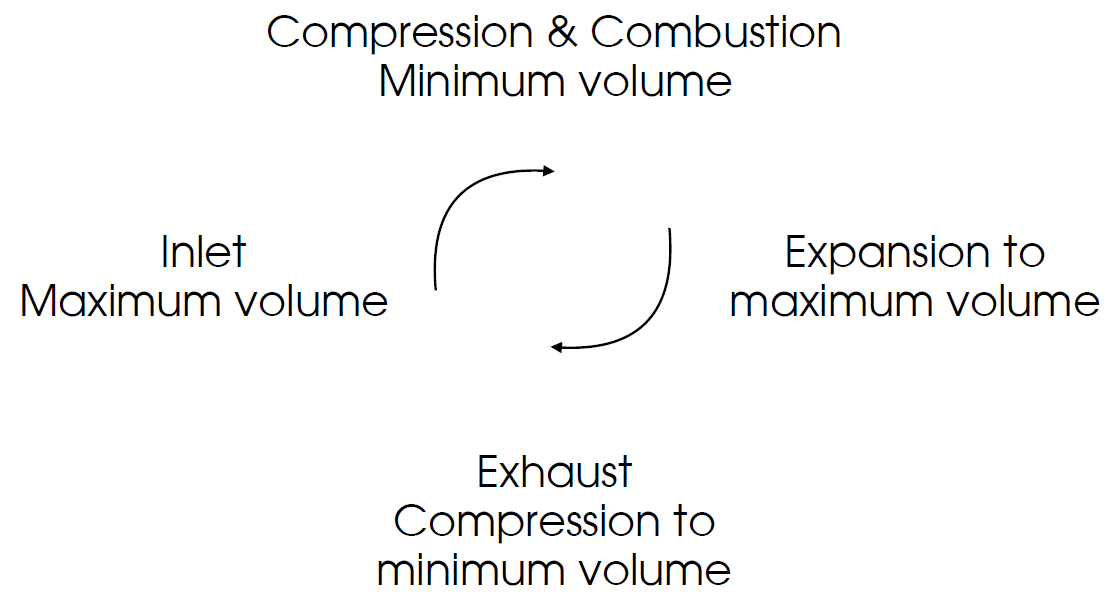
\includegraphics[scale=0.3]{ch1/1}
	\captionof{figure}{}
	\label{fig:1.1}
	\end{wrapfigure}
	Let's consider the integral on a moving volume of a function depending on time and position $f(\vec{x},t)$. Imagine that \autoref{fig:1.1} represents the moving volume at initial time containing mass $m$. An infinitesimal part of that volume contains an infinitesimal mass $dm = \rho dV$, where $\rho$ is mass density. We deduce the expression of the total mass at any time by that of the initial time  
	\begin{equation}
		M(t_0) = \int _{V(t_0)}\rho (\vec{x},t_0)\, dV \qquad \Rightarrow M(t) = \int _{V(t)}\rho (\vec{x},t)\, dV
	\end{equation}
	By considering $\rho (\vec{x},t)$ as $f(\vec{x},t)$, the derivative of the integral is given by
	
	\begin{center}
	\theor{\textbf{Reynolds transport theorem}
	\begin{equation}
		\frac{d}{dt}\int _{V(t)}f (\vec{x},t)\, dV = \int _{V(t)} \frac{\D f}{\D t} (\vec{x},t)\, dV + \oint _{S(t) = \D V(t)} f(\vec{x},t) \vec{b}\, \vec{n}\, dS
	\end{equation}
	where $\vec{b}$ is the surface displacement velocity. }
	\end{center}
	
	The second equation that will be used in the developement is given by
	\begin{center}
	\theor{\textbf{Gauss theorem}
	\begin{equation}
		\oint _{S = \D V} \vec{a} \, \vec{n} \, dS = \int _V \nabla \vec{a}\, dV
	\end{equation}}
	\end{center}
	
	\subsection{Mass conservation equation}
	If $V(t)$ is the moving volume occupied by the closed system as time varies, then by definition of a closed system $\frac{dM(t)}{dt} = 0$. The corresponding equation using Reynolds transport theorem is 
	\begin{equation}
		M(t) = \int _{V(t)} \rho\, dV \qquad \Rightarrow \frac{dM(t)}{dt} = \int _{V(t)} \frac{\D \rho}{\D t}\, dV + \oint _{S(t) = \D V(t)} \rho\, \vec{b}\, \vec{n}\, dS = 0
	\end{equation}
	\begin{wrapfigure}[9]{l}{3cm}
	\vspace{-5mm}
	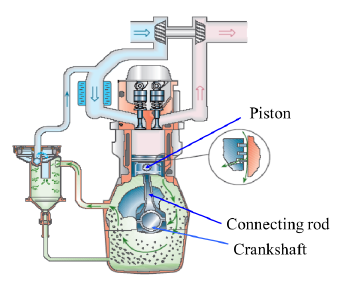
\includegraphics[scale=0.3]{ch1/2}
	\captionof{figure}{}
	\label{fig:1.2}
	\end{wrapfigure}
	We have to express that this volume is not traversed by material. There is no flux of fluid and the particles in the volume are always the same. By definition, the infinitesimal distance traveled by the surface and the fluid are
	\begin{equation}
		d\vec{x} = \vec{b}\, dt \qquad and \qquad d\vec{x}' = \vec{u}\, dt
	\end{equation}	 
	where $\vec{u}$ is the fluid velocity. Under wich condition do we know that the fluid has not traversed the boundary? We have to define the relative dispolacement $d\vec{x}'-d\vec{x}$ of the fluid in regard to the fluid. For a closed system 
	\begin{equation}
	\begin{aligned}
		(d\vec{x}'-d\vec{x})\cdot \vec{n} = 0 \quad &\Leftrightarrow \quad dt (\vec{u}-\vec{b})\cdot \vec{n} = 0 \quad \Leftrightarrow \quad (\vec{u}-\vec{b})\cdot \vec{n} = 0 \\
		&\Rightarrow \quad \vec{b} \vec{n} = \vec{u} \vec{n}
		\end{aligned}
	\end{equation}
	\begin{center}
	\theor{\textbf{Mass conservation equation for closed systems (integral form)}
	\begin{equation}
		\int _{V(t)} \frac{\D \rho}{\D t}\, dV + \oint _{S(t) = \D V(t)} \rho\, \underbrace{\vec{b}\, \vec{n}}_{=\vec{u}\, \vec{n}}\, dS =0
		\label{eq:1.7}
	\end{equation}}
	\end{center}
	
	How to write this equation in a different way? Let's consider now a fixed open system composed of fluid particles in the fixed volume $V_0(t) = V(t_0)$. Similarly to the previous point, the mass variation in this fixed volume is expressed like 
	\begin{equation}
		M_0(t) = \int _{V_0(t)} \rho\, dV \qquad 
		\Rightarrow \int _{V_0(t)} \frac{\D \rho}{\D t}\, dV + \oint _{S_0(t) = \D V_0(t)} \rho\, \vec{b}\, \vec{n}\, dS.
	\end{equation}
	The volume integral expresses the variable mass in the fixed volume and the surface integral is nul due to the nul surface velocity (since the volume is fixed). This relation enables us to write the 
	\begin{center}
	\theor{\textbf{Mass conservation equation for fixed open systems (integral form)}
	\begin{equation}
		\frac{dM_0}{dt} + \underbrace{\oint _{S_0(t) = \D V_0(t)} \rho\, \vec{u}\, \vec{n}\, dS = 0}_{\mbox{mass flow out of the system}}
	\end{equation}}
	\end{center}	
	Let's finally consider an arbitrary open system containing fluid particles in a moving volume $V_*(t)$ such that $V_*(t_0) = V(t_0) = V_0$. Similarly we have using the Reynolds transport theorem
	\begin{equation}
		M_*(t) = \int _{V_*(t)} \rho\, dV \qquad \Rightarrow \frac{dM_*(t)}{dt} = \int _{V_*(t)} \frac{\D \rho}{\D t}\, dV + \oint _{S_*(t) = \D V_*(t)} \rho\, \vec{b}\, \vec{n}\, dS
	\end{equation}
	Using the definition of the volume at $t=t_0$, we can equalize the volume integral with that of \eqref{eq:1.7} to find 
	\begin{center}
	\theor{\textbf{Mass conservation equation for arbitrary open systems (integral form)}
	\begin{equation}
		\frac{dM_*(t_0)}{dt} + \oint _{S(t_0) = \D V(t_0)} \rho (\vec{u}-\vec{b})\, \vec{n}\, dS = 0
	\end{equation}}
	\end{center}	
	
	Let's now take \eqref{eq:1.7} again and apply Gauss theorem
	\begin{equation}
	\begin{aligned}
		\int _{V(t)} \frac{\D \rho}{\D t}\, dV + \oint _{S(t) = \D V(t)} \rho \underbrace{\vec{u}\, \vec{n}}_{\vec{a}}\, &dS =0 \qquad with \qquad 
		\oint _{S(t)} \rho\, \underbrace{\vec{u}\, \vec{n}}_{\vec{a}}\, dS = \int _{V(t)} \nabla \rho \vec{u} \, dV \\
		&\Leftrightarrow \int _{V(t)} \left[ \frac{\D \rho}{\D t} + \nabla \rho \vec{u} \right] \,dV = 0
		\end{aligned}
	\end{equation}
	For this last equation to be true for all systems, the integrated term must be equal to zero 
	\begin{center}
	\theor{\textbf{Mass conservation equation (differential form (1) - divergent form)}
	\begin{equation}
		\frac{\D \rho}{\D t} + \nabla \rho \vec{u} = 0
		\label{eq:1.13}
	\end{equation}}
	\end{center}
	
	\begin{wrapfigure}[4]{l}{4cm}
	\vspace{-5mm}
	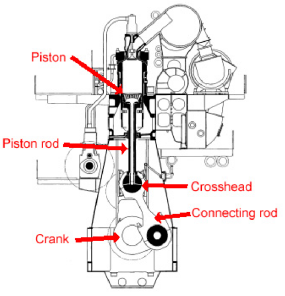
\includegraphics[scale=0.35]{ch1/3}
	\captionof{figure}{}
	\label{fig:1.3}
	\end{wrapfigure}
	In order to find the second differential form, let's consider 2 points Q and P as described in \autoref{fig:1.3}. The difference of density between the 2 points is \\\\\\
	\begin{equation}
	\begin{aligned}
		\rho _Q(t+dt) - \rho _P(t) &= \rho (x_1+dx_1,x_2+dx_2,x_3+dx_3,t+dt) - \rho (x_1,x_2,x_3)  \\
		&= d\rho = \frac{\D \rho}{\D x_1}dx_1 + \frac{\D \rho}{\D x_2}dx_2 + \frac{\D \rho}{\D x_3}dx_3 + \frac{\D \rho}{\D t}dt
		\end{aligned}
		\label{eq:1.14}
	\end{equation}
	In general, the fluid particles at $P(t)$ and $Q(t+dt)$ are different. However, if $dx_1 = u_1 dt, dx_2 = u_2 dt, dx_3 = u_3 dt$, then the fluid particles at the 2 points are the same. By making appear these velocities in \eqref{eq:1.14}, 
	\begin{equation}
		d\rho = \left( \frac{\D \rho}{\D x_1}u_1 + \frac{\D \rho}{\D x_2}u_2 + \frac{\D \rho}{\D x_3}u_3 + \frac{\D \rho}{\D t}\right) dt
	\end{equation}
	Finally, after dividing by $dt$ the 2 members of the equation, we obtain the definition of the time rate of change of density when I follow the fluid $\dot{\rho}$. As \eqref{eq:1.13} can be expressed in term of indicial notation like 
	\begin{equation}
		\frac{\D \rho}{\D t} + u_i \frac{\D\rho}{\D x_i} + \rho \frac{\D u_i}{\D x_i} = 0 
	\end{equation}
	Replacing the sum of first and second term by $\dot{\rho}$ gives the last form
	\begin{center}
	\theor{
	\textbf{Mass conservation equation (differential form (2) - substancial form)}
	\begin{equation}
	\dot{\rho} + \rho \nabla \vec{u} = 0
	\label{eq:1.17}
	\end{equation}
	}
	\end{center}
	
	\subsection{Newton's second law : Momentum equation}
	\begin{wrapfigure}[8]{l}{4cm}
	\vspace{-5mm}
	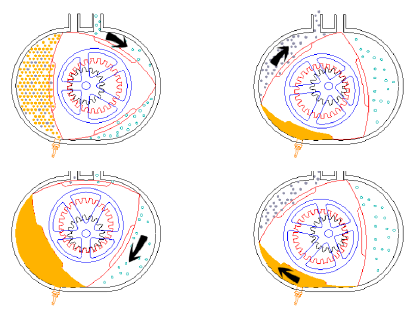
\includegraphics[scale=0.3]{ch1/4}
	\captionof{figure}{}
	\label{fig:1.4}
	\end{wrapfigure}
	Momentum in this course is noted $\vec{P}(t)$. For closed systems,
	\begin{equation}
		\frac{d\vec{P}(t)}{dt} = \sum \vec{F} = \frac{d}{dt}\int _{V(t)} \rho \vec{u}\, dV
		\label{eq:1.18}
	\end{equation}
	where $\rho \vec{u}$ is the momentum density. We will spell out the expression of the 2 members. First, the derivative, using the Reynolds transport theorem gives 
	\begin{equation}
		\frac{d\vec{P}}{dt} = \int _{V(t)} \frac{\D \rho \vec{u}}{\D t}\, dV + \oint _{S(t) = \D V(t)} \rho \vec{u} (\vec{u} \vec{n}) \, dS
	\end{equation}
	This written in indicial notation
	\begin{equation}
	\begin{aligned}
		\frac{dP_i}{dt} &= \int _{V(t)} \frac{\D \rho u_i}{\D t}\, dV + \oint _{S(t) = \D V(t)} \underbrace{\rho u_i u_j}_{tensor :\, \vec{u} \otimes \vec{u}} n_j \, dS\\
		&= \int _{V(t)} \frac{\D \rho u_i}{\D t}\, dV + \oint _{S(t) = \D V(t)} \rho (\vec{u} \otimes \vec{u}) \vec{n}\, dS 
		\end{aligned}
	\end{equation}
	and by applying Gauss theorem to the surface integral

	\begin{center}
	\begin{equation}
		\frac{d\vec{P}}{dt} = \int _{V(t)} \left[\frac{\D \rho \vec{u}}{\D t} + \nabla \rho \vec{u} \otimes \vec{u} \right] dV \qquad and \qquad \frac{dP_i}{dt} = \int _{V(t)} \left[ \frac{\D \rho u_i}{dt} + \frac{\D}{\D x_j} (\rho u_i u_j) \right] dV
	\end{equation}
	\end{center}
	
	Based on the previous forms, we can generalize this for any arbitrary function $\phi$
	\begin{equation}
	\begin{aligned}
		\frac{d}{dt} \int _{V(t)} \rho \phi\, dV  &= \int _{V(t)} \left[\frac{\D \rho \phi}{\D t} + \frac{\D}{\D x_j} \rho \phi u_j \right] dt \\
		&= \int _{V(t)} \left[ \rho \frac{\D \phi}{dt} + \phi \right. \underbrace{\left( \frac{\D \rho}{\D t} + \frac{\D \rho u_j}{\D x_j} \right)}_{= 0\ \eqref{eq:1.13}}\left. + \rho u_j\frac{\D \phi}{\D x_j} \right] dV \\
		&= \int _{V(t)} \rho \left[ \frac{\D \phi}{\D t} + u_j \frac{\D \phi}{\D x_j} \right] dV
	\end{aligned}
	\end{equation}
	Similarly to thermodynamics courses, we can introduce an extensive variable $\Phi$ and an intensive $\phi$ to have 
	\begin{center}
	\theor{
	\textbf{General relation for any arbitrary function in closed systems}
	\begin{equation}
		\frac{d\Phi }{dt} = \int _{V(t)} \left[ \frac{\D \rho \phi}{\D t} + \nabla \rho \phi \vec{u} \right] dV = \int _{V(t)} \rho \dot{\phi} \, dV
	\end{equation}
	}
	\end{center}
	For the specific case where $\Phi = \vec{P}$ and $\phi = \vec{u}$, we obtain
	\begin{equation}
		\frac{d\vec{P}}{dt} = \int _{V(t)} \rho \underbrace{\left[ \frac{\D \vec{u}}{\D t} + \vec{u} \nabla \vec{u} \right]}_{\dot{u}} dV 
		\label{eq:1.24}
	\end{equation}
	We can now express the forces applied on the system. There are 2 main classes : \\
	\begin{itemize}
		\item[•] \textbf{Distance forces (volume)} $\vec{F}_V$ : \\
		This type of force allows a body to influence another without being in contact with. 
		\begin{itemize}
			\item The most present one is gravity which is applied on each fluid particles ($d\vec{F} = dm \vec{g}$). We can imagine that there exists a force density $\vec{f}$ such that 
		\begin{equation}
			\vec{F}_V = \int _{V(t)} \vec{f} \, dV = \int _{V(t)} \rho \vec{a} \, dV
			\label{eq:1.25}
		\end{equation}
		where $\vec{a}$ is a force per unit mass, so an acceleration (gravity : $\vec{f} = \rho \vec{g}$). 
		
			\item If we have an electric material, we can talk about electromagnetic forces, which can be modelled as 
		\begin{equation}
			\vec{f} = \rho _c (\vec{E}+\vec{u}\times \vec{B}) + \vec{J}\times \vec{ B}
		\end{equation}
		where $\rho _c$ is the charge density $[C/m^3]$ and the second term is the Lorentz force. Indeed, if we have a lot of particles, we can talk of an average velocity $\vec{v}_k = \vec{u}+\vec{C}_k$, where $C_k$ is a particular velocity due to molecular agitation.  The force applied on the system is 
		\begin{equation}
			\vec{F}_k = q_k [\vec{E} + \vec{v}_k \times \vec{B}] \qquad \Leftrightarrow \qquad \underbrace{\frac{\sum \vec{F}_k}{V}}_{\rho _c} = \frac{\sum q_k}{V} (\vec{E}+\vec{u}\times \vec{B}) + \underbrace{\frac{\sum q_k \vec{C}_k}{V}}_{\vec{J}} \times \vec{B}
		\end{equation}
		Mollecules are in general neutral, but containing non-neutral regions. Fluids are essentially neutral, $\vec{F}_V = 0$ in most cases. They are called quasi-neutral fluids. Electric influenced fluids will not be considered in that course but they existence has to be known. 
		
			\item They are also entrainment and Coriolis forces in rotating frame of references. These forces due to the rotation of Earth are not considered due to the small rotative velocity, unlike pomps and turbines. \\
		\end{itemize}
		\item[•] \textbf{Contact forces (surface)} $\vec{F}_S$ : \\
		
		\begin{minipage}{0.23\textwidth}
		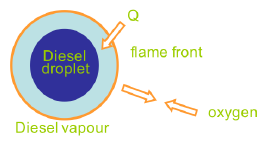
\includegraphics[scale=0.3]{ch1/5}
		\captionof{figure}{ }
		\label{fig:1.5}
		\end{minipage}
		\begin{minipage}{0.7\textwidth}
		These forces results from the contact of an internal and external fluid in regard of a region of surface $dS(t)$. We have 
		\begin{equation}
			d\vec{F}_S = \vec{T}\, dS \qquad \Rightarrow \vec{F}_S = \oint _S \vec{T}\, dS
			\label{eq:1.28}
		\end{equation}
		$\vec{T}$ is a force per unit area, a continuous function of space depending on location $\vec{x}$ and also linearly on the infinitesimal surface orientation $\vec{n}$. If $\vec{T}$ is the force per unit area for a surface element normal
		\end{minipage}
		 to the unit vector in the $j$ direction $e_j$, $\vec{T}(\vec{x}) = \vec{T}_jn_j$. \eqref{eq:1.28} becomes
		 \begin{equation}
		 \vec{F}_S = \oint _S \vec{T}_j n_j \, dS \qquad and \qquad F_{S_i} = \oint _S \underbrace{\tau _{j,i}}_{\sigma _{ji}} n_j\, dS 
		 \label{eq:1.29}
		 \end{equation}
		 where $\sigma _{ji}$ is the stress tensor. 
		\end{itemize}
		We can now take \eqref{eq:1.18} and replace the terms using \eqref{eq:1.24}, \eqref{eq:1.25} and \eqref{eq:1.29} to obtain the 
		
		\begin{center}
		\theor{\textbf{Momentum equation (integral form)}
		\begin{equation}
			\frac{dP_i}{dt} = \int _{V(t)} \left[\frac{\D \rho u_i}{\D t} + \nabla \rho u_i \vec{u} \right] dV = \int _{V(t)} \rho \dot{u}\, dV = \int _{V(t)} \rho a_i\, dV + \oint _{S(t)} \sigma _{ji} n_j \, dS
			\label{eq:1.30}
		\end{equation}
		}
		\end{center}
		We can see that $\sigma _{ji}$ and $\rho u_iu_j$ have the same mathematical nature. This is not surprising because in fact these forces result from molleculare agitation in fluids. Let's discuss it. We said that $\vec{v}_k = \vec{u} + \vec{C}_k$. Let's consider a surface element and make the hypothesis that the fluid is in rest, so the average velocity $\vec{u} = 0$. It doesn't mean that the particles are immobile, but that if all particles have the same mass (pure fluid) and if a certain number of particles are going from right to left with velocity $\vec{c}$, there are the same number of particles going from left to right with velocity $-\vec{c}$. There is no global mass flux. So for n particles going in one direction, the mass flux
		\begin{equation}
			2nm\vec{u} = nm\vec{c} + 2nm(-\vec{c}) = 0 
		\end{equation}
		To obtain the momentum in direction $x_1$, we have to multiply the mass flow in this direction by the velocity in this direction 
		\begin{equation}
			nm (\vec{c}\cdot \vec{e_1})c_1 + nm (-\vec{c_1}\cdot \vec{e_1})(-c_1) = 2nmc_1^2
		\end{equation}
		The global momentum flux traversing the unit surface is so positive going out of the volume. We need so a balance force in the opposite direction to keep the mass in. This explains the presence and nature of $\sigma _{ji}$ which is a momentum flux. \\
	Let's finally establish the differential form of the momentum equation, applying Gauss theorem to the second right side of \eqref{eq:1.30}
	\begin{equation}
		\int _{V(t)} \rho a_i\, dV + \oint _{S(t)} \sigma _{ji} n_j \, dS = \int _{V(t)} \left[ \rho a_i + \frac{\D \sigma _{ji}}{\D x_j} \right] dV
	\end{equation}
	and by considering the whole equation
	\begin{equation}
		\int _{V(t)} \left[ \frac{\D \rho u_i}{\D t} + \frac{\D \rho u_i u_j}{\D x_j} - \rho a_i - \frac{\D \sigma _{ji}}{\D x_j} \right] dV = 0 = \int _{V(t)} \left[ \rho \dot{u}_i - \rho a_i - \frac{\D \sigma _{ji}}{\D x_j} \right] dV
	\end{equation}
	and for this to be true for all systems we consider, we obtain
	\begin{center}
		\theor{\textbf{Momentum equation (differential form (1) - divergent form)}
		\begin{equation}
			\frac{\D \rho u_i}{\D t} + \frac{\D \rho u_i u_j}{\D x_j} = \rho a_i + \frac{\D \sigma _{ji}}{\D x_j} \qquad and \qquad \frac{\D \rho \vec{u}}{\D t} + \nabla \rho \vec{u}\otimes \vec{u} = \rho \vec{a} + \nabla \bar{\bar{\sigma}}
			\label{eq:1.35}
		\end{equation}
		}
		\end{center}
		
	\begin{center}
		\theor{\textbf{Momentum equation (differential form (2) - substancial form)}
		\begin{equation}
			\rho a_i + \frac{\D \sigma _{ji}}{\D x_j} = \rho \dot{u}_i \qquad and \qquad \rho \vec{a} + \nabla \bar{\bar{\sigma}} = \rho \dot{\vec{u}}
			\label{eq:1.36}
		\end{equation}
		}
		\end{center}
		
	\subsection{Angular momentum equation}
		This is a corollary of the momentum equation that states that \textit{the time rate of change of the angular momentum of a closed system is equal to the sum of the torques applied to the system.} There is no additional information except that the stress tensor should be symetric 
		\begin{equation}
			\sigma _{ji} = \sigma _{ij}
		\end{equation}
		
	\subsection{Energy equation - First principle of thermodynamics}
		If we note $\mathcal{E}$ the total energy of the system, the first principle tells that
		\begin{equation}
			\frac{d\mathcal{E}}{dt} = \dot{W} + \dot{Q}
			\label{eq:1.38}
		\end{equation}
		where $\dot{W}$ is the mechanical power provided by the forces applied on the system and $\dot{Q}$ the thermal power provided to the system. We will proceed like the previous equation expressing first the left side then the right side. If we note $E$ the total energy per unit mass, $e$ the internal energy per unit mass and $k$ the kinetic energy per unit mass (potential energy is not considered in order not to take into account power coming from potential forces)
		\begin{equation}
			\mathcal{E} = \int _{V(t)} E\, dm = \int _{V(t)} \rho E \, dV = \int _{V(t)} \rho (e+k) \, dV \qquad with \quad k = \frac{\vec{u} \vec{u}}{2}
		\end{equation}
		The time derivative of the energy using the Reynolds transport theorem, then the Gauss theorem is 
		\begin{equation}
		\begin{aligned}
			\frac{d\mathcal{E}}{dt} &= \int _{V(t)} \frac{\rho (e+k)}{dt} \, dV + \oint _{S(t)} \rho (e+k)\vec{u} \vec{n} \, dS \\
			&= \int _{V(t)} \left[\frac{\rho (e+k)}{dt} + \nabla \rho (e+k)\vec{u}  \right] dV = \int _{V(t)} \rho \dot{(e+k)}\, dV 
		\end{aligned}
		\label{eq:1.40}
		\end{equation}
		Let's now go on with with the mechanical power expression. We expressed in \eqref{eq:1.30} that there are volume and surface forces. These multiplied by the velocity and using Gauss gives 
		\begin{equation}
			\dot{W} = \int _{V(t)} \rho a_i u_i \, dV + \oint _{S(t)} \sigma _{ji} u_i n_j \, dS = \int _{V(t)} \left[ \rho a_i u_i + \frac{\D}{\D x_j}\sigma _{ji} u_i\right] dV
			\label{eq:1.41}
		\end{equation}
		\begin{wrapfigure}[6]{l}{3cm}
		\vspace{-5mm}
		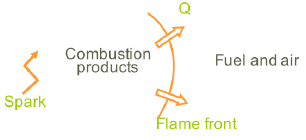
\includegraphics[scale=0.3]{ch1/6}
		\captionof{figure}{}
		\end{wrapfigure}
		For the thermal power expression, we need to introduce a new concept that is the heat flux vector $\vec{q}$ which qualifies a thermal power per unit area leaving the surface. Physically, there is only two heat transport mecanism which are radiation and conduction. Indeed, convection is a specific conduction case where the temperature gradient region becomes thinner and favorises the exchange. The thermal power is 
		\begin{equation}
			\dot{Q} =  - \oint _{S(t)} \vec{q} \vec{n} \, dS = - \int _{V(t)} \nabla \vec{q} \, dV
			\label{eq:1.42}
		\end{equation}
		Replacing the terms of \eqref{eq:1.38} by \eqref{eq:1.40}, \eqref{eq:1.41} and \eqref{eq:1.42} gives 
		\begin{center}
		\theor{
		\textbf{Total energy equation (integral form)}
		\begin{equation}
			\int _{V(t)} \frac{\rho (e+k)}{dt} \, dV + \oint _{S(t)} \rho (e+k)\vec{u} \vec{n} \, dS = \int _{V(t)} \rho \vec{a}\vec{u} \, dV + \oint _{S(t)} (\bar{\bar{\sigma}} \vec{n}) \vec{u}\, dS - \oint _{S(t)} \vec{q} \vec{n} \, dS
		\end{equation}
		}
		\end{center}
		
		The differantial form is obtained using Gauss theorem for the two sides and regrouping all the terms into one integral
		\begin{equation}
		\begin{aligned}
			&\int _{V(t)} \left[\frac{\rho (e+k)}{dt} + \nabla \rho (e+k)\vec{u} - \rho \vec{a} \vec{u} - \nabla \bar{\bar{\sigma}}\vec{u} + \nabla \vec{q} \right] dV = 0 \\
			\Leftrightarrow \qquad &\int _{V(t)} \left[\rho\dot{(e+k)} - \rho \vec{a} \vec{u} - \nabla \bar{\bar{\sigma}}\vec{u} + \nabla \vec{q} \right] dV = 0
		\end{aligned}
		\end{equation}
		
		And considering the fact that this has to be true for all systems, we obtain the two last forms
		\begin{center}
		\theor{
		\textbf{Total energy equation (differential form (1) - divergent form)}
		\begin{equation}
			\frac{\rho (e+k)}{dt} + \nabla \rho (e+k)\vec{u} = \rho \vec{a} \vec{u} + \nabla \bar{\bar{\sigma}}\vec{u} - \nabla \vec{q}
		\end{equation}
		}
		\end{center}
		\begin{center}
		\theor{
		\textbf{Total energy equation (differential form (2) - substantial form)}
		\begin{equation}
			\rho \dot{(e+k)} = \rho (\dot{e} + \dot{k}) = \rho \vec{a} \vec{u} + \nabla \bar{\bar{\sigma}}\vec{u} - \nabla \vec{q}
			\label{eq:1.46}
		\end{equation}
		}
		\end{center}
		Let's finally establish the distribution of the forces in the different energies. If we multiply \eqref{eq:1.36} by velocity $\vec{u}$ and if we observe that $\dot{k} = \frac{\dot{u}_i u_i+u_i\dot{u}_i}{2} = u_i \dot{u}_i$, we obtain 
		
		\begin{center}
		\theor{
		\textbf{Kinetic - Mechanical energy equation}
		\begin{equation}
			\vec{u}\left(\rho a_i + \frac{\D \sigma _{ji}}{\D x_j} = \rho \dot{u}_i\right) \qquad \Leftrightarrow \qquad \rho \underbrace{u_i \dot{u}_i}_{\dot{k}} = \rho u_i a_i + \frac{u_i \D\sigma _{ji}}{\D x_j}
			\label{eq:1.47}
		\end{equation}
		}
		\end{center}
		The difference between total energy \eqref{eq:1.46} and kinetic energy \eqref{eq:1.47} gives the internal energy
		
		\begin{center}
		\theor{
		\textbf{Internal energy equation}
		\begin{equation}
			\rho \dot{e} = 0 + \sigma _{ji} \frac{\D u_i}{\D x_j} - \nabla \vec{q} 
			\label{eq:1.48}
		\end{equation}
		}
		\end{center}
		We see that volume forces only contributes to the kinetic energy, heat flux only to the internal energy and the suface forces to both. 
		
	\subsection{Summary - Complementary equation}
		Let's make the inventory of the 3 substancial equations that we found. How many equations and unknowns do we have? 
	\begin{itemize}
		\item[•] In continuity equation \eqref{eq:1.17}, $\rho$ and $u_i$ are 4 unknowns in 3D. 
		\item[•] In momentum equation \eqref{eq:1.36}, $a_i$ is an external applied force so is known, $\sigma _{ji}$ consists in 6 unknowns (symetric matrix).
		\item[•] In internal energy equation \eqref{eq:1.48}, $e$ and $\vec{q}$ are 4 most unknowns. 
	\end{itemize}			
	\ \\
	The total unknowns number is 14.  The number of disponible equations is 5, 1 thanks to the energy, 1 thanks to the continuity and 3 thanks to the vectorial momentum equation. In this stage, we haven't made any assumption on the nature of the material we're considering. These equations are valid for an elastic solid as a fluid. The main difference is that solids resist to a deformation whereas fluid doesn't. But fluid resists to a rate of deformation. The way that stress tensor $\sigma _{ji}$ is related to the displacement field is called the constitutuve equations. 
	
	\subsubsection{Constitutive relations} 
		For a fluid, the stress tensor depends on the fluid rate of deformation (rate of strain). To express $\sigma _{ji}$, we have to find a quantity in the field of motion of the fluid that represents the rate of strain. If the velocity field $\vec{u}(\vec{x},t)$ was uniform, not depending on $\vec{x}$, the fluid will be moving as a bulk and there is no rate of deformation. The rate of strain must be somehow related to the velocity gradient tensor $\nabla \otimes \vec{u}$. We know that all tensors can be decomposed in an antisymetric and symetric part like 
		\begin{equation}
			\nabla \otimes \vec{u} = \frac{\D u_j}{\D x_i} = \Omega _{ji} + S _{ij} = \frac{1}{2} \left( \frac{\D u_j}{\D x_i} - \frac{\D u_i}{\D x_j} \right) + \frac{1}{2} \left( \frac{\D u_j}{\D x_i} + \frac{\D u_i}{\D x_j} \right).
		\end{equation}
		
		For a constant gradient velocity field, the velocity field is linear in the coordinates
		\begin{equation}
			u_j = \frac{\D u_j}{\D x_i}x_i = \Omega _{ji} x_i + S _{ij} x_i
			\label{eq:1.51}
		\end{equation}
		
		Let's look to the mathematical nature of the antisymetric part.  If we express using Kronecker $\delta$, we have
		\begin{equation}
			\Omega _{ji} =\frac{1}{2} \left( \frac{\D u_j}{\D x_i} - \frac{\D u_i}{\D x_j} \right) = \frac{1}{2} \delta _{kij}\delta _{kqp} \frac{\D u_p}{\D x_q} \qquad 
			with \quad \delta _{kij}\delta _{kqp} = \delta _{iq}\delta _{jp} - \delta _{ip}\delta _{jq} 
		\end{equation}
		Knowing that $(a \times b)_k = \delta _{kpq} a_p b_q$, we can introduce the \textbf{curle} (rotationnel) of velocity called vorticity $\vec{\omega}$
		\begin{equation}
			\delta _{kqp} \frac{\D u_p}{\D x_q} = (\nabla \times \vec{u})_k \qquad \Rightarrow \nabla \times \vec{u} = \vec{\omega}
		\end{equation}		 
		Let's look to the way this is linked to \eqref{eq:1.51}
		\begin{equation}
			 u_j^{AS} = \Omega _{ji}x_i = \frac{1}{2} \delta _{jki} \omega _k x_i = \frac{1}{2} (\vec{\omega} \times \vec{x})_j
			\qquad \Leftrightarrow \qquad 
			\vec{u}^{AS} = \frac{1}{2} \vec{\omega}\times \vec{x}
		\end{equation}
	 	In conclusion, we see that the antisymetric part consists in a pure rotation velocity field, a rigid body motion of angular velocity $\frac{1}{2}\vec{\omega}$ without strain. $\vec{\omega}$ is twice the angular velocity of fluid particles around themselves. The quantity representative of the fluid rate of strain can only be the symetric part of the velocity gradient tensor called the rate of strain tensor. For a fluid, $\sigma _{ij} = f(S_{ij})$. \\
	 	
	  To determine the nature of this relationship, we will assume that $\sigma _{ij} $ is a linear function of $S_{pq}$. This is called 
	\begin{center}	  
	\theor{
	  \textbf{Newton's assumption for stresses}
	  \begin{equation}
	  	\sigma _{ij} = a_{ij} + b_{ijpq} S_{pq}.
	  \end{equation}
	  }
	  \end{center}
	  In this equation, $b_{ijpq}$ is a tensor with four indices, but we know that it's symetric with respect to $pq$ and $ij$ because $S$ is symetric with respect to $pq$ and $ij$, leading to $6 \times 6 = 36$ coefficients. Symetric tensor $a_{ij}$ counts 6 coefficients, for a total of 42 coefficients. \\
	  If we assume that the fluid is \textbf{isotropic}, meaning that the fluid react in the same way whatever the sollicitation direction. For example, let's take a case of $S_{ij}$ where all coefficients are null except the $S_{11}$ term. Diagonal terms reprensent a rate of elongation/stretch while the off-diagonal terms represent an angular deformation between two perpendicular direction. The assumption means that if the rate of stress is not in 1 direction but 2, the fluid reaction will be the same. In other words, if we make a rotation of coordinates, the relation in the rotated frame of reference must be the same. In that case, the relation reduces to
	  \begin{equation}
	  	\sigma _{ij} = a \delta _{ij} + bS _{ij} + c \delta _{ij}S_{kk}
	  	\label{eq:1.55}
	  \end{equation}
	  where only 3 coefficient must be found. It is natural to think that air and water have no preferential direction unlike certain solid as wood that has a preferential direction related to the orientation of fibers. Blood or dissolved polymer chains are examples of non isotropic fluids. We will from now consider the fluid to be isotropic. \\
In \eqref{eq:1.55} $a$ is a constant that represents the stress present when the fluid is at rest. 	The surface force associated to that component is purely normal 
		\begin{equation}
			\sigma _{ij} n_j = a \delta _{ij} n_j = an_i
		\end{equation}
		This constant corresponds to the pressure exerted by the fluid at rest. Because of its application in the opposite direction to the normal, it's negative. The two other coefficients represents the 2 coefficients of viscosity
		\begin{equation}
			a = -p \qquad b = 2\mu \qquad c = \lambda
		\end{equation}
		The stress tensor equation can so be written with a pressure stress and a viscous stress part like 
		\begin{equation}
			\sigma _{ij} = -p\delta _{ij} + \tau _{ij} \qquad with \qquad \tau _{ij} = 2\mu S_{ij} + \lambda \delta _{ij} S_{kk}
			\label{eq:1.58}
		\end{equation}
	  	An alternative form to that is the following 
	  	\begin{equation}
	  		\tau _{ij} = 2 \mu \underbrace{\left( S_{ij} + \frac{1}{3} \delta _{ij} S_{kk} \right)}_{\equiv S_{ij}^S} +\underbrace{\left( \lambda + \frac{2\mu}{3} \right)}_{\equiv \mu _V} \delta _{ij} S_{kk}
	  	\end{equation}
	  	This notation is necessary to make appear the part of the strain tensor which has no trace $S_{ij}^S$, called the rate of shear. Indeed 
	  	\begin{equation}
	  		S_{ii}^S = S_{ii} - \frac{1}{3}\delta _{ii}S_{kk} = 0
	  	\end{equation}
	  	This means that $S_{ij}^S$ represents the trace less part of the rate of \textbf{strain} tensor called the sheer rate tensor. What is now $S_{kk}$ ? 
	  	\begin{equation}
	  		S_{kk} = \frac{1}{2} \left( \frac{\D u_k}{\D x_k} + \frac{\D u_k}{\D x_k} \right) = \frac{\D u_k}{\D x_k} = \nabla \vec{u}
	  	\end{equation}
	  	The divergence of the velocity is related to the rate of dilatation of the fluid, the change of volume. We decomposed the rate of strain in a part representing the deformation without change of volume (pure deformation) and another with change of volume ($\mu _V$ is the bulk viscosity). Another expression for $\tau _{ij}$ with a final net gain of 3 unknowns is 
	  	\begin{equation}
	  		\tau _{ij} = 2 \mu S_{ij}^S + \mu _V \delta _{ij} \nabla \vec{u}
	  		\label{eq:1.62}
		\end{equation}	  	 
		At this stage, we have to determine still 6 unknowns from the 9 at the beginning. 
		
	\subsubsection{Heat flux}
		We discussed about the fact that heat flux propagates using 2 physical mechanism : conduction and radiation. In the energy equation it's the divergence of the heat fluc that appears. In most application, the radiative effect does not imply heat accumulation or loss. The fluids are so transparent to radiative heat flux $\nabla \vec{q}^{rad} =0$. We only have conduction and the Fourier law says that 
		\begin{equation}
			\vec{q} \propto \nabla T = d\nabla T = -\kappa \nabla T \qquad \Leftrightarrow \qquad q_i = -\kappa \frac{\D T}{\D x_i}
		\end{equation}
	The negative sign comes from the fact that heat goes from hot to cold (decrease of T). We have a net gain of 1 unknown with this equation. 
	
	\subsubsection{Thermodynamics}
		At this stage, we are using 4 thermodynamics intensive variables which are $\rho, e, p, T$. We know that for a single phase fluid, the variance is 2, meaning that we can use 2 thermodynamics equations of state (EoS) relating them. For example, for a alorically and thermally perfect gas, we will have 
		\begin{equation}
			p = \rho R T \qquad and \qquad e = c_v T
		\end{equation}		 
		We have a net gain of 2 unknows, so there remains 2 unknowns.  
		
	\subsubsection{Transport coefficients}
		The remaining variables are the shear viscosity $\mu$, the bulk viscosity $\mu _V$ and thermal conductivity $\kappa$. These are functions of the thermodynamic state. For example for gases we have the relations 
		\begin{equation}
			\mu = f(T) \qquad and \qquad Pr = \frac{\mu c_p}{\kappa} = cst \Leftrightarrow \kappa = \frac{\mu (T) c_p (T)}{Pr}
		\end{equation}
		The bulk viscosity is more difficult to determine, but it can be shown that for monoatomic gases (no internal degres of freedom) $\mu _V=0$. For diatomic gases it's much more delcate to measure, but it has been shown that for many flows, the flows is insensitive to the variation of value of bulk viscosity. In fact, for fluids without divergence of velocity, we don't care about $\mu _V$ because there is no variation of volume  \eqref{eq:1.62}. We will so make the following assumption
		\begin{center}
		\theor{\textbf{Stokes assumption}
		\begin{equation}
			\mu _V = 0 \quad \mbox{even for other gases}.
		\end{equation}
		}
		\end{center}
		 We're done, we have as many equations as variables. We mentioned the first principle of thermodynamics but not the second. Let's analyse that. 
		 
		\subsubsection{Second principle of thermodynamics}
			We will reuse the internal energy equation \eqref{eq:1.48}, replace $\sigma _{ij}$ by it's expression in \eqref{eq:1.58} and use the fact that $\frac{\D u_i}{\D x_j} = \Omega _{ij} + S_{ij}$
			\begin{equation}
				\rho \dot{e} = \sigma _{ij} \frac{\D u_i}{\D x_j} - \frac{\D q_i}{\D x_i} = -p \delta _{ij} \frac{\D u_i}{\D x_j} + (2\mu S_{ij}^S + \mu _V \delta _{ij} \nabla \vec{u})(S_{ij}+\cancel{\Omega _{ij}}) - \frac{\D q_i}{\D x_i}
			\end{equation}
			where $\Omega _{ij}$ doesn't contribute because the contraction of the symetric tensor by the antisymetric tensor is equal to 0.  We have the relation 
			\begin{equation}
			S_{ij}^S = S_{ij}-\frac{1}{3}\delta _{ij}\nabla \vec{u} \qquad \Leftrightarrow \qquad S_{ij} = S_{ij}^S + \frac{1}{3}\delta _{ij}\nabla \vec{u}
	  		\end{equation}
	  		Combined to the fact that $\delta _{ij} \frac{\D u_i}{\D x_j} = \frac{\D u_i}{\D x_i} = \nabla \vec{u}$, we obtain
	  		\begin{equation}
	  			\rho \dot{e} = -p \nabla \vec{u} + (2\mu S_{ij}^S + \mu _V \delta _{ij} \nabla \vec{u})\left( S_{ij}^S + \frac{1}{3}\delta _{ij}\nabla \vec{u}\right) - \nabla \vec{q}
	  		\end{equation}
	  		The mass conservation equation tells us that we can write the divergence as 
	  		\begin{equation}
	  			\dot{\rho} + \rho \nabla \vec{u} = 0 \qquad \Leftrightarrow \qquad \nabla \vec{u} = -\frac{\dot{\rho}}{\rho} = -\rho \left( \frac{\dot{\rho}}{\rho ^2}\right) = \rho \dot{\left( \frac{1}{\rho}\right)} = \rho \dot{v}
	  		\end{equation}
	  		If we replace the divergence in the previous equation, we have
	  		\begin{equation}
	  			\rho \dot{e} = -\rho p \dot{v} + (2\mu S_{ij}^S + \mu _V \delta _{ij} \nabla \vec{u})\left(S_{ij}^S + \frac{1}{3}\delta _{ij}\nabla \vec{u}\right) - \nabla \vec{q}
	  		\end{equation}
	  		The first term here looks like the reversible work $-pdv$ in thermodynamics and is so the reversible contribution to the internal energy. Let's make this appear by bringing this to the left side. We make appear $\rho [\dot{e} + p\dot{v}]$, but we have the famous Gibbs relation $de = Tds - pdv \Leftrightarrow \dot{e} = T\dot{s}-p\dot{v}$. We have now 
	  		\begin{equation}
	  			\rho \dot{s} = \frac{(2\mu S_{ij}^S + \mu _V \delta _{ij} \nabla \vec{u})\left(S_{ij}^S + \frac{1}{3}\delta _{ij}\nabla \vec{u}\right)}{T} - \frac{\nabla \vec{q}}{T}
	  			\label{eq:1.72}
	  		\end{equation}
	  		If we remind the relation we demonstrated before for any variable $\dot{\Phi} = \int _V \rho \dot{\phi} dV$, we can make the analogy here to say that when this is integrated over a volume, it gives the time rate of change of the entropy of the closed system that's initially inside this volume. We have to identify the reversible part in this equation. We know that the reversible entropy rate of exchange for a uniform system and its integral over a closed surface is given by
	  		\begin{equation}
	  			\frac{\vec{q}dS}{T} \qquad \Rightarrow \qquad \oint _S \frac{\vec{q}}{T}(-\vec{n})\, dS = -\int _V \nabla \frac{\vec{q}}{T} \, dV.
			\end{equation}	  		 
			We see that we have to make appear a this in the last equation. But we know that
			\begin{equation}
				\frac{\nabla \vec{q}}{T} = \nabla \frac{\vec{q}}{T} - \vec{q} \nabla \left(\frac{1}{T} \right) = \nabla \frac{\vec{q}}{T} + \vec{q} \frac{\nabla T}{T^2}
			\end{equation}
			And by introducing this into the relation \eqref{eq:1.72}, we make appear the reversible entropy rate of exchange
			\begin{equation}
				\rho \dot{s} = -\nabla \frac{\vec{q}}{T} - \frac{\vec{q}\nabla T}{T^2} + \frac{(2\mu S_{ij}^S + \mu _V \delta _{ij} \nabla \vec{u})\left(S_{ij}^S + \frac{1}{3}\delta _{ij}\nabla \vec{u}\right)}{T}
			\end{equation}
			We also know that $\vec{q} = -\kappa \nabla T$, making appear $(\nabla T)^2$
			\begin{equation}
				\rho \dot{s} = -\nabla \frac{\vec{q}}{T} + \frac{\nabla T\nabla T}{T^2} + \frac{(2\mu S_{ij}^S + \mu _V \delta _{ij} \nabla \vec{u})\left(S_{ij}^S + \frac{1}{3}\delta _{ij}\nabla \vec{u}\right)}{T}
			\end{equation}
			If we imagine a fluid at rest with only a heat exchange operating on it, the third term $=0$, the first term is reversible so anyway the sign and the second term must be positive. This implies $\kappa \geq 0$ due to the square of the other varaibles (the heat has to go from hot to cold). Let's expand the third term
			\begin{equation}
				\rho \dot{s} = -\nabla \frac{\vec{q}}{T} + \frac{\nabla T\nabla T}{T^2} + \frac{1}{T}\left[ 2\mu S_{ij}^S S_{ij}^S + \cancel{\mu _V \nabla \vec{u} \delta _{ij} S_{ij}^S} + \cancel{2\mu S_{ij}^S \frac{\delta _{ij}}{3} \nabla \vec{u}} + \mu _V \frac{\delta _{ij}\delta _{ij}}{3}(\nabla \vec{u})^2  \right]			
			\end{equation}			 
			In this last equation, the second and third terms are nul because $S_{ii}^S=0$. Let's imagine that we have a fluid with only dilation and no shear $S_{ij}^S$, the last term must be positive and so $\mu _V$ has to be positive ($\geq 0$). In the other hand, for the first term, we have a quadratic form (sum of squares $\geq 0$), so $\mu$ has to be positive. To verify the second principle, we have to verify these 3 inequalities. In fluid mechanics, we don't have to worry about the second principle, it's built in the equations as long as the transport coefficient are positive.  
			
	\subsection{Boundary conditions}
		We have now to establish the boundary conditions which makes the difference between the flow cases. First of all, we have two main categories of flows : 
		\begin{itemize}
			\item[•] \textbf{External flows} (unbounded domain)\\
				For example, a flow over a wing, assuming that atmosphere extends to infinity. In that case we have far field boundary conditions, what happens far from the body ($u\rightarrow u_\infty, p\rightarrow p_\infty, T\rightarrow T_\infty)$. 
			
			\item[•] \textbf{Internal flows} (bounded domain)\\
				For example, a flow in a pipe or a fluid in a rotating machine like a pump. In that case we don't have the far field conditions but the inlet and outlet boundary conditions but this problem is not discussed here. 
		\end{itemize}
		
		\subsubsection{Solid surfaces}
			In both case we have solid surfaces, we have to make a distinction. We wrote the equation for the general case of a viscous flow, but there is flows where the viscous stresses can be neglected (not $=0$ !) leading to what we call the \textbf{inviscid flows}. Let's analyse the two cases. 
			
		\subsubsection{Viscous flows}
			Viiscosity is associated to the exchange of momentum between neighboring fluid layers due to molecular agitation. If we have a molecule coming from a low velocity region to a high velocity region, it slows down the molecule there and inversely. The same occurs when a fluid particle enter in contact with solid surfaces, it exchange momentum. The result is that velocity and temperature fields must be continuous 
			\begin{equation}
				\vec{u}_{fluid} = \vec{u}_{wall} \qquad and \qquad T_{fluid} = T_{wall}
			\end{equation}
			In particular, for a surface at rest, the fluid must be at rest on the solid surface as well. This is called the \textbf{no-slip condition}. 
		
		\subsubsection{Inviscid flows} 
			For inviscid flows, this mecanism doesn't exist, the fluid may slip. The boundary condition is that the fluid can't go throw the solid
			\begin{equation}
				\vec{u}_{fluid}\vec{n} = \vec{u}_{wall}\vec{n}
			\end{equation}
			This is called the \textbf{slip/no penetration condition}. The previous condition is stronger because in fact $\vec{u} = \vec{u}_n\vec{n}+\vec{u}_t$ includes the tangential condition too. 
			
\section{Special cases}
	\subsection{General case}
		The generale equations are the following : 
		\begin{itemize}
			\item[•] Mass conservation equation 
			\begin{equation}
				\dot{\rho} + \rho \nabla \vec{u} = 0 
			\end{equation}
			
			\item[•] Momentum equation
			\begin{equation}
				\rho \dot{\vec{u}} = - \nabla p + \nabla \bar{\bar{\tau}} + \rho \vec{F}
			\end{equation}
			
			\item[•] Energy equation
			\begin{equation}
				\rho \dot{e} = - p \nabla \vec{u} + \underbrace{\bar{\bar{u}} .. \nabla \otimes \vec{u}}_{\epsilon _V} - \nabla \vec{q}
			\end{equation}
			where $\nabla \otimes \vec{u}$ can be replace by the symetric part, rate of strain tensor $\bar{\bar{S}}$ and $\epsilon _V$ is the viscous dissipation. \\
			
			\item[•] Constituve relation
			\begin{equation}
			\begin{aligned}
				\tau _{ij} &= 2\mu \left( S _{ij} - \frac{1}{3}\delta_{ij}\nabla \vec{u} \right) + \mu _V S_{ij}\nabla \vec{u}\\
				&= \mu \left( \frac{\D u_i}{\D x_j} + \frac{\D u_j}{\D x_i} - \frac{2}{3}\delta _{ij}\nabla \vec{u} \right) + \mu _V S_{ij}\nabla \vec{u}
			\end{aligned}
			\label{eq:1.83}
			\end{equation}
			
			\item[•] Conductive heat flux 
			\begin{equation}
				\vec{q} = -\kappa \nabla T
			\end{equation}
		\end{itemize}
		
	\subsection{Steady flow} 
		This is caracterized by the fact that $\frac{\D }{\D t} = 0$ and implies for example that 
		\begin{equation}
			\dot{\rho} = \frac{\D \rho}{\D t} + \vec{u} \nabla \rho = \vec{u} \nabla \rho
		\end{equation}
		and for the others. 
		
	\subsection{Inviscid flows}
		They are defined as flows in which vicous stresses and conduction heat flux can be neglected.  We are talking about flows and not fluids because there is no fluid with $\mu = 0$ or $\kappa = 0$. This happens for superfluids but we don't care. When we look at the fluid properties tables, in SI units, water and air have very small $\mu$ but we can't say that there are negligible because it depends on the system of refference used. If something is negligible  it is with respect to something else. Let's start with the viscous stresses. Momentum equation can be written as 
		\begin{equation}
			\rho \dot{\vec{u}} = \frac{\D \rho}{\D t} + \nabla \rho \vec{u} \otimes \vec{u} = -\nabla p + \nabla \bar{\bar{\tau}} + \rho \bar{F}
		\end{equation}
		where the viscous stress tensor is a tensor as the momentum flux tensor. They correspond to the same physical phenomenon but at different scales, the viscous stress tensor is due to the molecular agitation whereas the momentum flux tensor is for the macroscopic scale, the average scale. So it makes sense to compare the order of magnitude of the two ones. \\
		
		\begin{wrapfigure}[6]{l}{4cm}
		\vspace{-8mm}
		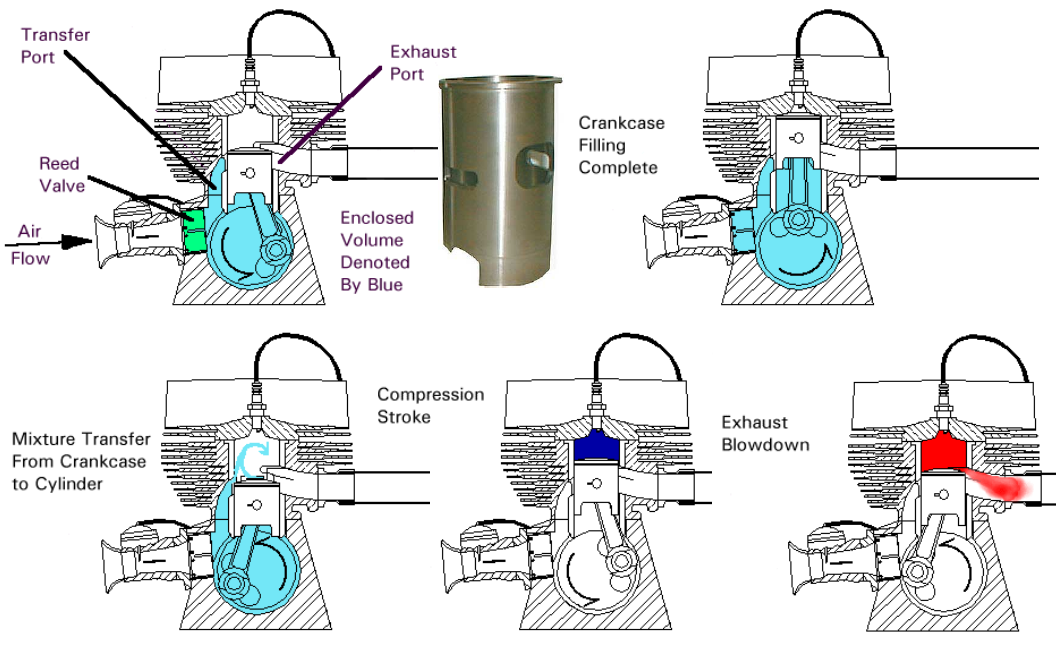
\includegraphics[scale=0.38]{ch1/7}
		\captionof{figure}{}
		\end{wrapfigure}
		Let's consider a fluid flows of far field velocity $\vec{U}$ around a solid body of characteristic lenght $L$, if we consider the momentum flux tensor, we know that the velocity around the body will vary between 0 and $U$ so the order of magnitude will be $\theta (\rho U^2)$. What about $\tau$? We see that in \eqref{eq:1.83} appears the velocity gradient, derivative. What is the order of magnitude of the derivative of a function?  
		
		\begin{wrapfigure}[8]{l}{3.5cm}
		\vspace{-5mm}
		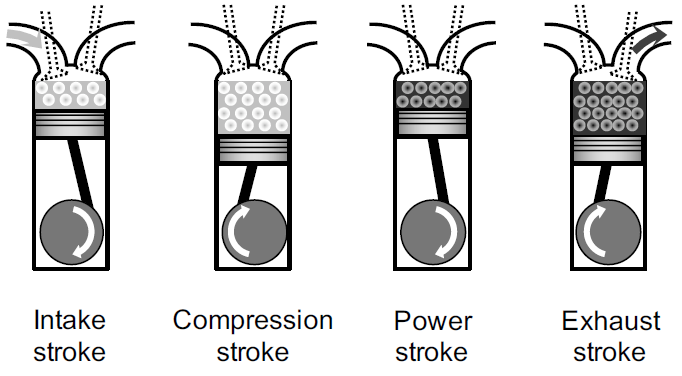
\includegraphics[scale=0.5]{ch1/8}
		\captionof{figure}{}
		\label{fig:1.8}
		\end{wrapfigure}
		Let's consider a function $f(x)$ represented on \autoref{fig:1.8}. If the function is smooth, so if the function doesn't vary much in the interval, its derivative keeps a constant order of magnitude in the integral. We see it in the figure, the slope varies between $a$ and $b$, can be twice the slope at the center but keeps the same order of magnitude. So for a smooth function, the order of magnitude of $f'$ remains the same over the interval $f' = \theta \left(\frac{\Delta f}{\Delta x}\right)$. Let's use this to have an approximation for the velocity gradient tensor 
		\begin{equation}
			\nabla \otimes \vec{u} = \theta \left( \frac{U}{L} \right) \qquad \Rightarrow \bar{\bar{\tau}} = \theta \left( \mu \frac{U}{L} \right)
		\end{equation}
		The relative order of magnitude of viscous stresses with respect to momentum flow is 
		\begin{equation}
			\frac{\mu \frac{\cancel{U}}{L}}{\rho U^{\cancel{2}}} = \frac{\mu}{\rho UL} = \frac{1}{Re_L}
		\end{equation}
		We conclude that viscous stresses can be neglected in the case of high Reynolds number. \\
		
		\begin{wrapfigure}[7]{r}{3.5cm}
		\vspace{-8mm}
		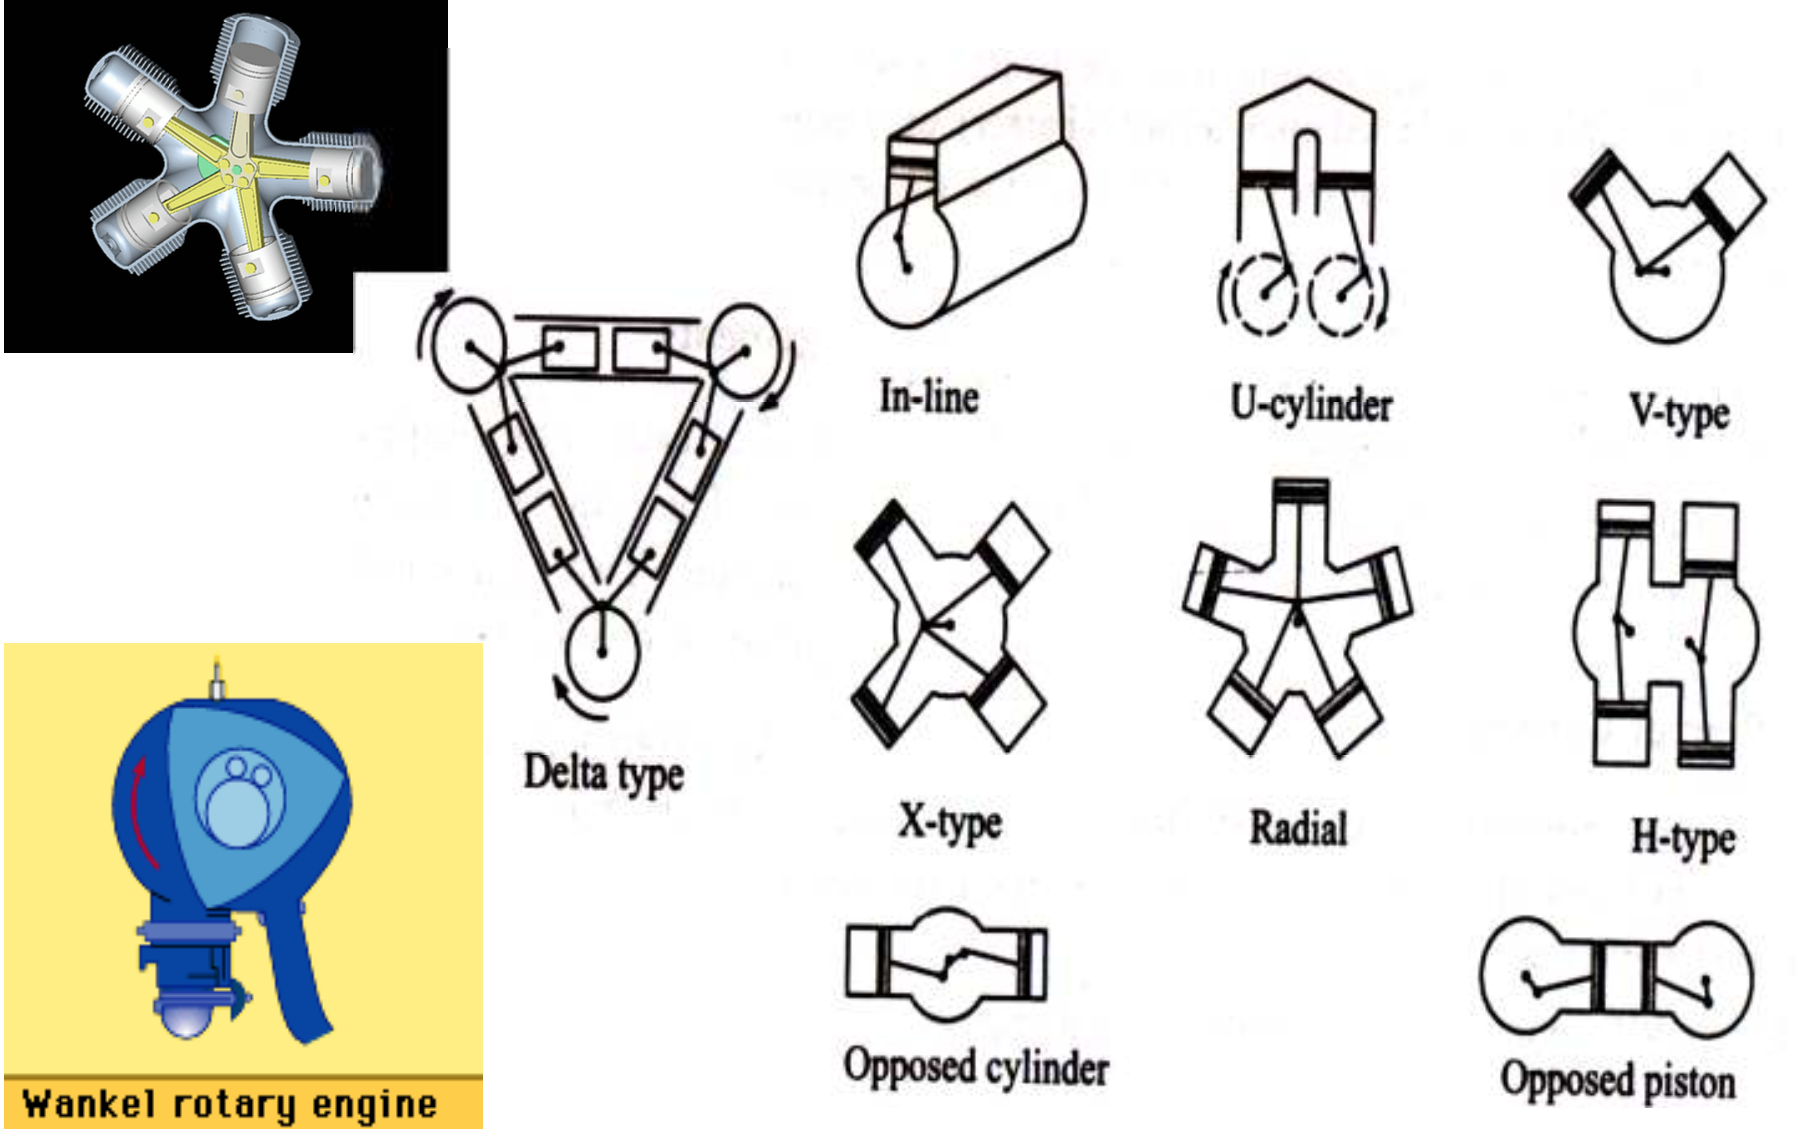
\includegraphics[scale=0.53]{ch1/9}
		\captionof{figure}{}
		\label{fig:1.9}
		\end{wrapfigure}
		Now we have to verify the assumption that velocity is a smooth function of the coordinates. Examples of not smooth functions are represented on \autoref{fig:1.9} where the green curve is smooth close to the limits but not smooth in a small interval and the yellow one is a periodic function with the characteristic wave length. In these cases, $\Delta x$ is not the appropriate length scale to determine the order of magnitude of the derivative. \\\\\\

		\begin{wrapfigure}[6]{l}{4cm}
		\vspace{-15mm}
		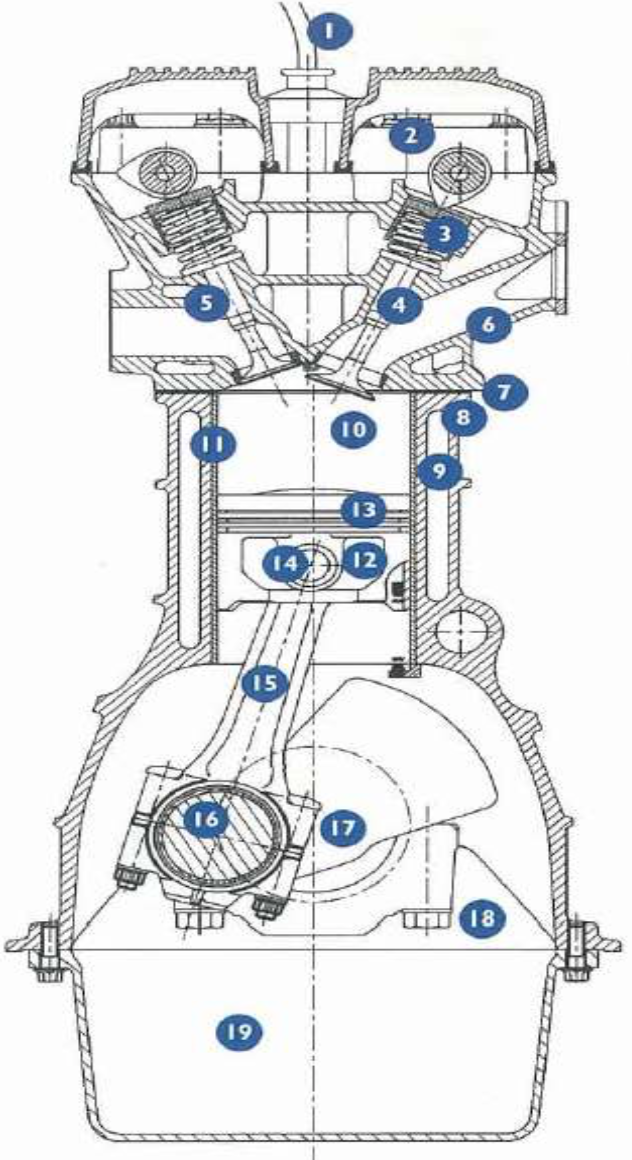
\includegraphics[scale=0.35]{ch1/10}
		\captionof{figure}{}
		\label{fig:1.10}
		\end{wrapfigure}
		Now what about the velocity field? Let's assume that velocity is smooth and the fluid inviscid, the boundary conditions to respect are the slip conditions. But we know that $\mu$ is not strictly 0, so the velocity must be 0 at the wall and therefore, there exists an area of rapidly changing velocity close to the wall. 
%%%%%%%%%%%%%%%%%%%%%%%%%%%%%%%%%%%%%
% Ch2 : Les liaisons interatomiques %
%%%%%%%%%%%%%%%%%%%%%%%%%%%%%%%%%%%%%

\chapter{Liaisons interatomiques}
\section{La liaison}
Le but des liaisons est de remplir la couche de valence et de se rapprocher au plus de la configuration des gaz rares. L'existence de composés polyatomiques stables implique que les atomes soient capable de former des agrégats dont \textbf{l'énergie est plus faible que s'ils étaient isolés}. Les types de liaison dépendent de l'agencement des électrons de valence et sont au nombre de 4 : \\

\begin{itemize}
	\item[•] la liaison ionique
	\item[•] la liaison covalente
	\item[•] la liaison métallique
	\item[•] les liaisons secondaires hydrogène et de Vander Waals. \\
\end{itemize}
	
Les 3 premières sont des liaisons fortes alors que les dernières sont plus faibles. Soulignons que, le plus souvent, la liaison des atomes dans un solide présente un caractère mixte associant des contributions simultanées de plusieurs types liaisons chimiques.
	
\section{La liaison ionique, opportunisme individualiste}
Type de liaison qui détermine la cohésion des solides constitués de l'association d'atomes possédant des affinités électronique très différentes. Prenons l'exemple du sel de cuisine $NaCl$ et regardons ce qui se passe d'un point de vue énergétique. Tout d'abord, l'énergie de première ionisation de $Na$ et l'affinité électronique (énergie libéré lorsqu'un électron est capté) de $Cl$ sont
\begin{equation}
	E_{ion}\, Na= 5.14 \, eV \qquad et \qquad \mbox{Aff.élec } Cl = 4.02 \, eV 
\end{equation}	 
ce qui veut dire qu'il faut $U_i = 1.12\, eV$ pour séparer $NaCl$ en $Na^++Cl^-$. Il faut encore tenir compte de la force électrostatique $F$ entre les deux ions de charges différentes. Quand un ion se rapproche depuis l'infini, 
\begin{equation}
	U_a = \int _\infty ^r F_{attr} \, dr= \int _\infty ^r \frac{q^2}{4\pi \epsilon _0 r^2} \, dr = -\frac{q^2}{4\pi \epsilon _0 r}
\end{equation}
Le signe négatif de cette énergie traduit le fait que les ions ont tendance à se rapprocher. Cependant, à très petite distance, les cortèges électroniques commencent à se superposer et une forte répulsion apparaît selon 
\begin{equation}
	U_r = \frac{B}{r^n}
\end{equation}
\begin{wrapfigure}[5]{l}{6.5cm}
	\vspace{-5mm}
	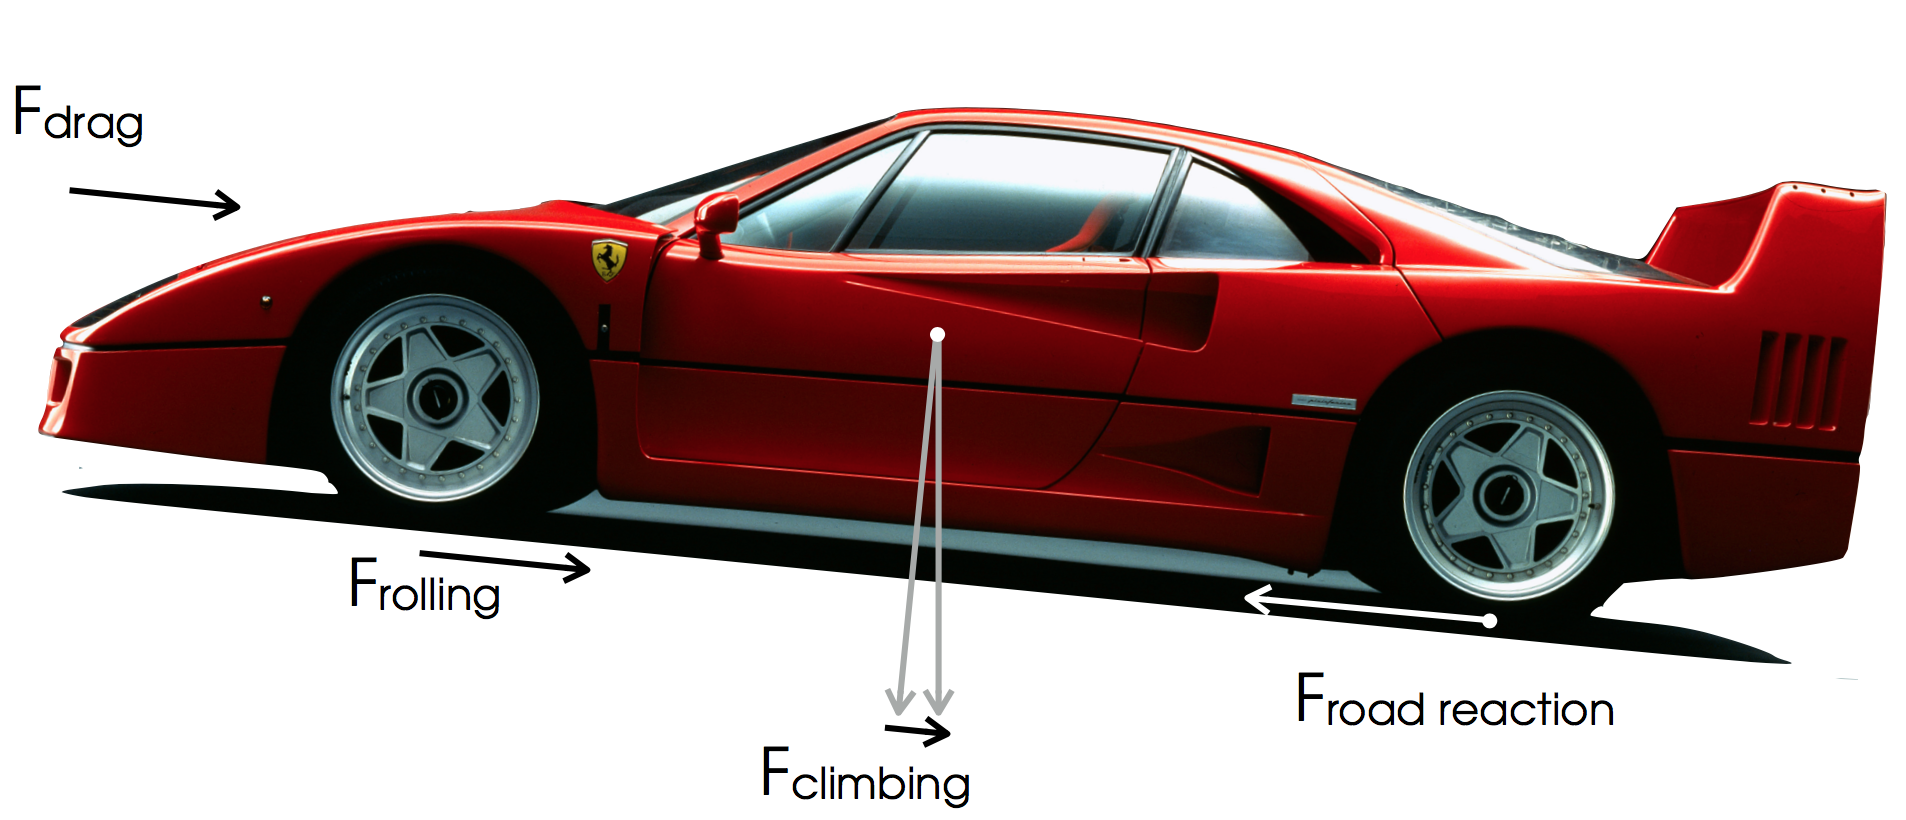
\includegraphics[scale=0.6]{ch2/1}
\end{wrapfigure}
La somme de toutes ces contributions donne la courbe d'énergie potentielle suivante. 
A SUIVRE
\chapter{Traction - Compression}
\section{Traction}
	\subsection{Méthode cinématique}
	\begin{wrapfigure}[8]{r}{6.5cm}
	\vspace{-5mm}
	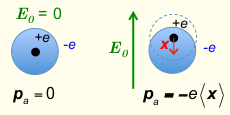
\includegraphics[scale=0.4]{ch3/image1.png}
	\captionof{figure}{ }
	\end{wrapfigure}
	Nous allons ici utiliser la méthode cinématique de sorte que les équations 
	de compatibilité soient satisfaites lors de l'obtention de notre relation 
	contrainte $\leftrightarrow N$. Il faut donc postuler un champ de 
	déplacement :
	\begin{equation}
	u = u_0(x),\qquad v=0,\qquad w=0.
	\end{equation}
	On considère un déplacement axial $u$, uniquement selon $x$ : ne varie 
	pas selon $x$ et $y$ et constante dans toute la section : une section 
	transversale plane, reste plane\footnote{hypothèse de Bernoulli (1694) :
	les sections droites initialement planes et perpendiculaires à l'axe le 
	restent dans la configuration déformée}.
	
	\subsection{Déplacements - Déformations - Contraintes}
		\subsubsection{Déformations}
		Maintenant que nous avons notre déplacement, il faut s'intéresser 
		aux déformations :
		\begin{equation}
		a_{ij} = \frac{1}{2}\left(\dfrac{\partial u_i}{\partial x_j}+\dfrac{
		\partial u_j}{\partial x_i}\right)
		\end{equation}
		De par notre champ, $\epsilon_x$ est constant dans la section 
		transversale et les autres composantes sont nulles :
		\begin{equation}
		\epsilon_x = \dfrac{\partial u_0}{\partial x}
		\end{equation}
		
		\subsubsection{Contraintes}
		On utilise pour ça la loi de Hooke $ \sigma_x = E\epsilon_x$. Notons 
		que si $E$ est constant, $\sigma_x$ l'est dans la section transversale.
		On néglige les composantes de Poisson.
		
	\subsection{Éléments de réduction : section homogène}
	La suite de notre méthode demande le calcul des éléments de réductions. 
	Supposons que l'on ai une section homogène de sorte que $E$ soit constant. 
	Dès lors, $\sigma_x$ est également constant. Pour la normale, c'est immédiat :
	\begin{equation}
	N = \int_A \sigma_x\ dA \qquad\Longrightarrow\qquad N = \sigma_xA
	\end{equation}
	En raison de notre champ uniquement selon $x$, les résultantes en $y$ et $z$ 
	sont nulles, de même pour le moment selon $x$\\
		\begin{wrapfigure}[7]{l}{6.5cm}
	\vspace{-5mm}
	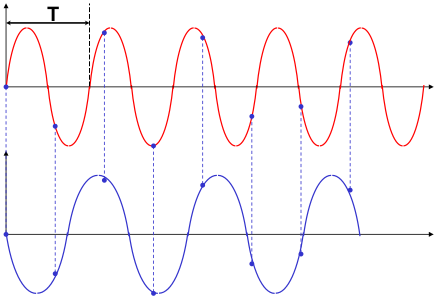
\includegraphics[scale=0.45]{ch3/image2.png}
	\captionof{figure}{ }
	\end{wrapfigure}
	\begin{equation}
	\begin{array}{ll}
	R_y = \int_A \tau_{xy}\ dA &\Longrightarrow T_y = 0\\
	\text{Similairement : }&\Longrightarrow T_z = 0\\
	C_x = \int_A (\tau_{xz}y-\tau_{xy}z)\ dA &\Longrightarrow M_x = 0
	\end{array}
	\end{equation}
	Pour le moment selon $y$ (et similairement pour $z$) nous avons :
	\begin{equation}
	C_y = \int_A \sigma_xz\ dA\qquad\Longrightarrow\qquad C_y =  \sigma_x
	\int_A z\ dA
	\end{equation}
	Si l'origine des axes est le \textbf{centre géométrique}\footnote{Centre 
	de "gravité" sans masse.} défini tel que 
	\begin{equation}
	\int_A y\ dA = 0,\qquad \int_A z\ dA = 0.
	\end{equation}
	ALors, $M_y$ et $M_z$ sont nuls.
	
		\subsubsection{En résumé}
		La poutre est uniquement soumise à un effort \textbf{normal} (et pas 
		un fléchissant). Pour une poutre de section homogène ($E$ constant), 
		nous avons une distribution uniforme de la contrainte axiale 
		\begin{equation}
		\sigma_x = \dfrac{aN}{A}
		\end{equation}
		Pour une poutre homogène à effort normal constant ($N$ constant) :
		\begin{equation}
		\epsilon_x = \dfrac{\Delta L}{L}\qquad\text{où}\quad \Delta L = 
		\dfrac{NL}{EA}
		\end{equation}
		L'hypothèse de Bernoulli est une hypothèse cinématique (\textit{Les 
		sections droites initialement planes et perpendiculaires à l'axe le
		restent dans la configuration déformée.}) et ne fait donc \textbf{pas} 
		intervenir les propriétés physiques du matériau.\\
		\danger Il n'y aura traction sans flexion \textbf{que si} les moments 
		des contraintes axiales sont nuls !
		
		
	\subsection{Éléments de réduction : section non homogène}		
	Si $E \neq\ cste$, les relations générales restent inchangées tant que 
	$E$ n'apparaît pas explicitement. Dès qu'il apparaît :
	\begin{equation}
	\sigma_x(x,y,z) = E(x,y,z)\epsilon_x(x)
	\end{equation}
	La répartition de $\sigma_x$ dans une section transversale ($x =\ cste$) 
	est dès lors donné par 
	\begin{equation}
	\sigma_x(y,z) = E(y,z)\epsilon_x
	\end{equation}
	Au niveau des éléments de réduction $R_{y,z}, M_{x,y,z}$ restent inchangés 
	(nuls\footnote{Si l'origine des axes est le centre géométrique!}). Par contre, 
	$N$ n'a plus la même expression, $\sigma_x$ n'étant plus constant.\\
	\textsc{Exemple} : slide 15-16.
	
\section{Les treillis articulés}
	\subsection{Hypothèses}
	Deux hypothèses sont d'application :
	\begin{enumerate}
	\item Il s'agit d'un ensemble de poutres rectilignes assemblées par des 
	nœuds articulés ne transmettant pas de couple (On peut tourner librement 
	l’extrémité)
	\item Les forces extérieures sont appliquées uniquement aux nœuds
	\end{enumerate}
	
	\subsection{Équilibre d'une poutre}
	Dans ce cas-ci, on ne dira pas "poutre" mais \textit{barre}. Celle-ci est 
	uniquement soumise à un effort normal $N$. Ses équations d'équilibres 
	s'obtiennent on ne peut plus facilement\\
	\begin{wrapfigure}[6]{l}{7.5cm}
	\vspace{-8mm}
	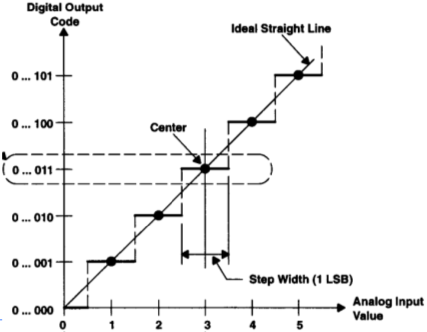
\includegraphics[scale=0.4]{ch3/image3.png}
	\captionof{figure}{ }
	\end{wrapfigure}
	\begin{equation}
	\left\{\begin{array}{ll}
	F_{xA} + F_{xB} &=0\\
	F_{yA} + F_{yB} &= 0\\
	LF_{yB} &=0
	\end{array}\right.
	\end{equation}\ \\
	
	
	\subsection{Équilibre des nœuds}
	\begin{wrapfigure}[7]{r}{6.5cm}
	\vspace{-4mm}
	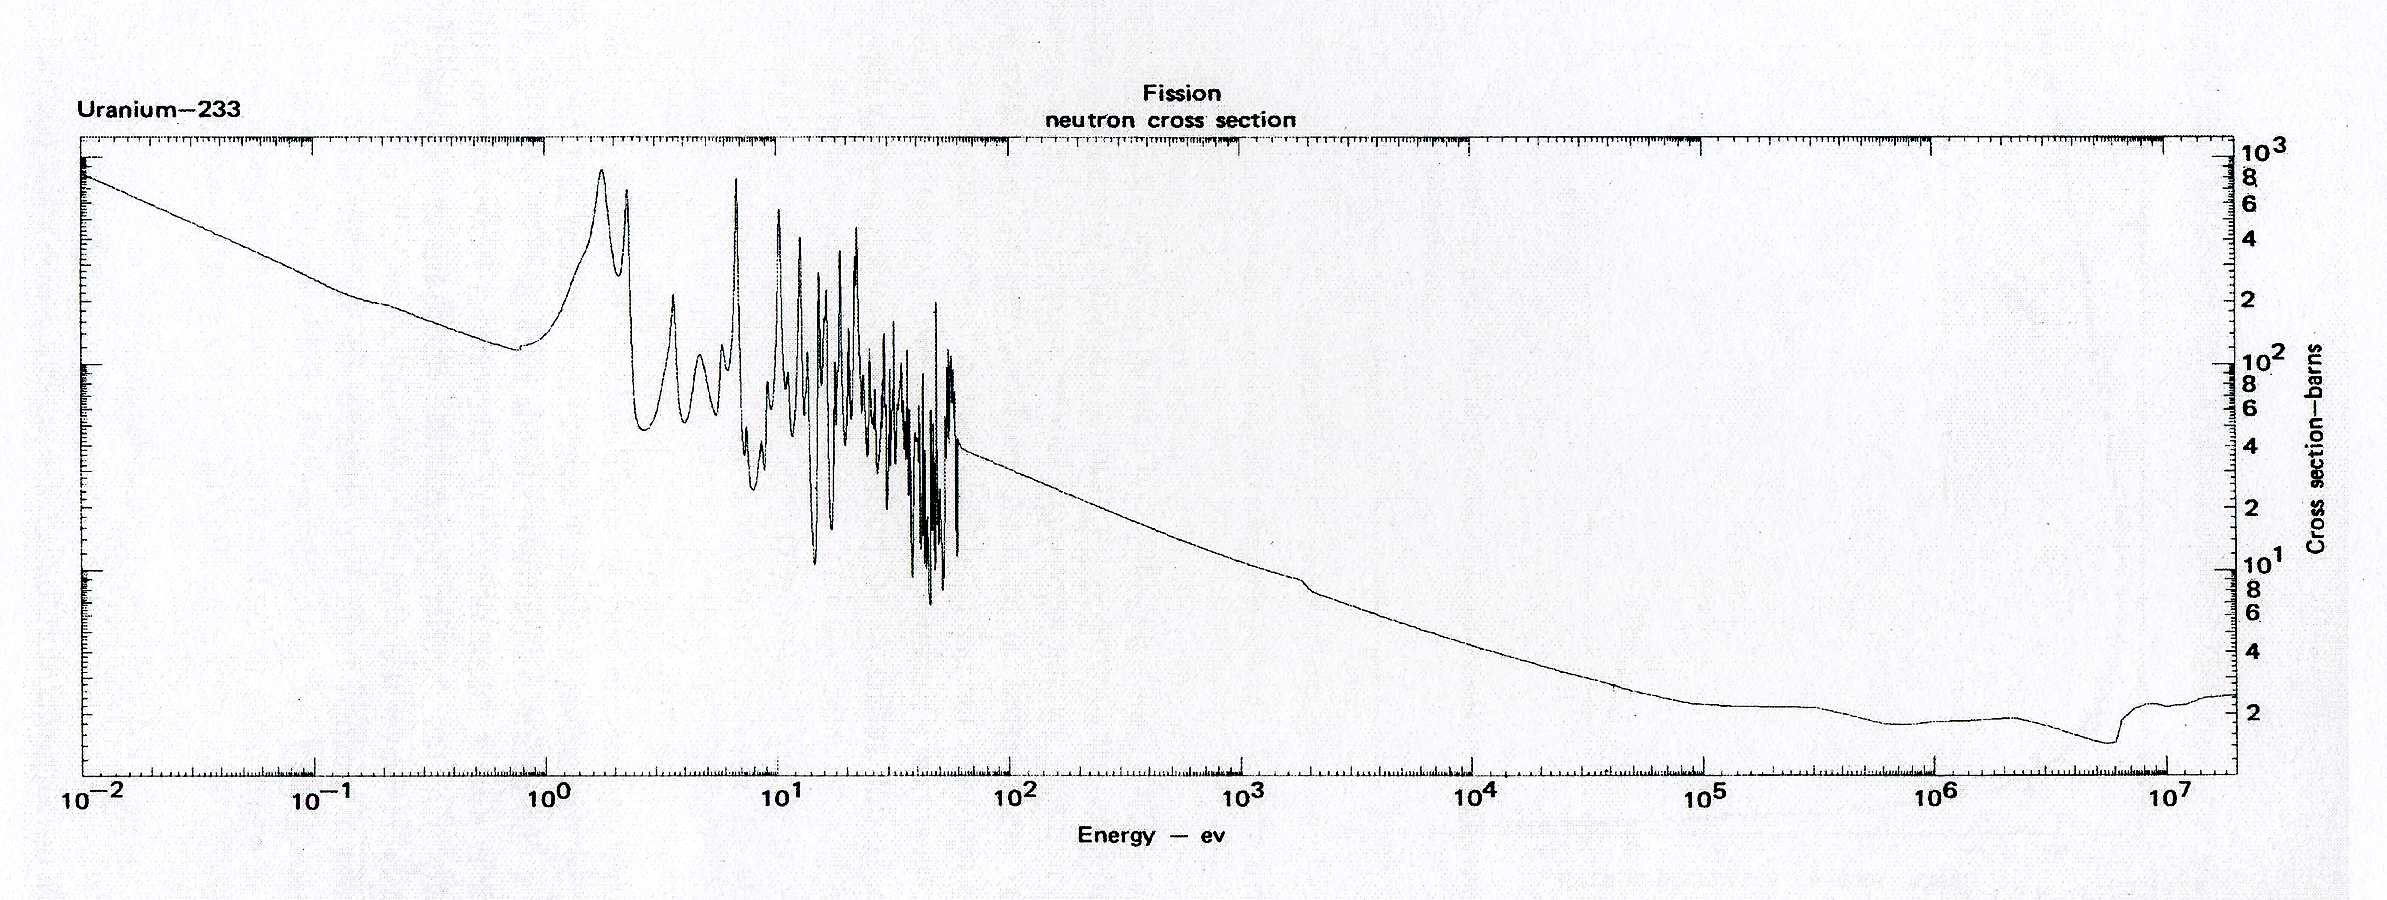
\includegraphics[scale=0.4]{ch3/image4.png}
	\captionof{figure}{ }
	\end{wrapfigure}
		Encore une fois rien de difficile, la méthode est systématique :
	\begin{itemize}
	\item[$\bullet$] Isoler un nœud en coupant les barres qui y aboutissent
	\item[$\bullet$] Appliquer les efforts normaux et les efforts extérieurs
	\item[$\bullet$] Écrire les équations d’équilibre du nœud
	\end{itemize}
	
	\subsection{Structure isostatique ?}
	La condition d'isostaticité est que le nombre d'inconnues statiques soit 
	égal au nombre d'équations d'équilibres. Nous avons :
	\begin{itemize}
	\item[$\bullet$] Nombre de barres : $b \rightarrow b$ efforts normaux 
	inconnus
	\item[$\bullet$] Nombre de RDL : $R \rightarrow R$ composantes de réactions 
	inconnues
	\item[$\bullet$] Nombre de nœuds : $n\rightarrow 2b$ équations d'équilibres 
	en 2D
	\end{itemize}
	Une structure est isostatique si (CN mais pas CNS) :
	\begin{equation}
	b + R = 2n
	\end{equation}
	\newpage
	
	\subsection{Coupe de Ritter}
		\subsubsection{Principe}
	\begin{wrapfigure}[7]{r}{7cm}
	\vspace{-4mm}
	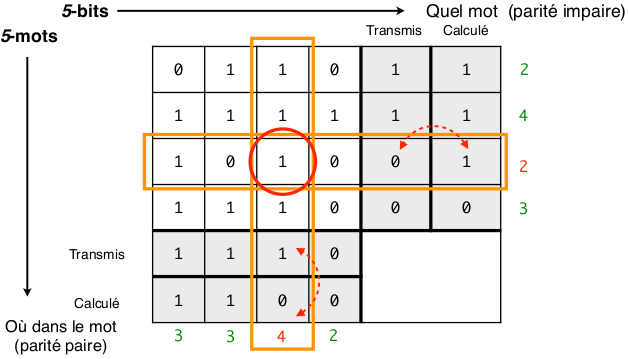
\includegraphics[scale=0.4]{ch3/image5.png}
	\captionof{figure}{ }
	\end{wrapfigure}
		On cherche à calculer l'effort normal dans une barre. On va
		\begin{itemize}
		\item[$\bullet$] Couper la structure en deux parties \textbf{disjointes}
		\item[$\bullet$] Écrire l'équilibre d'une des parties
		\item[$\bullet$] S'arranger que cet effort normal soit la seule inconnue
		\end{itemize}
		Les slides 24-25 montrent comment appliquer cette méthode.
		
	\subsection{Quelques nœuds particuliers}
	Certains nœuds particuliers permettent de gagner du temps dans les calculs.
	\begin{center}
	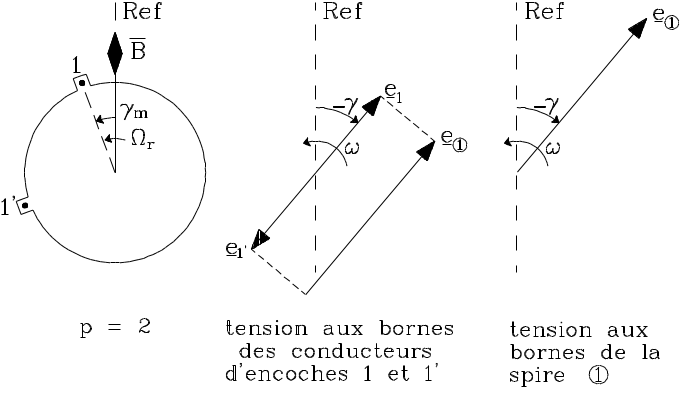
\includegraphics[scale=0.5]{ch3/image6.png}
	\captionof{table}{ }
	\end{center}
	
	
		\subsubsection{Barres à efforts nuls}
		\begin{wrapfigure}[9]{l}{7cm}
		\vspace{-6mm}
		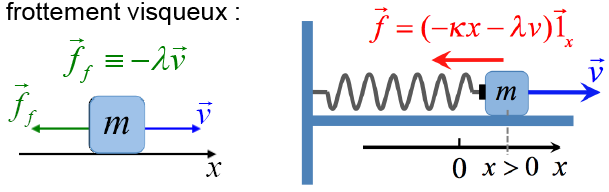
\includegraphics[scale=0.4]{ch3/image7.png}
		\captionof{figure}{ }
		\end{wrapfigure}
		En appliquant ce magnifique tableau et en l'appliquant sur la figure 
		ci-dessous, je peux déjà affirmer que pleins d'efforts normaux seront 
		nuls avant même de commencer à faire des calculs et donc gagner du 
		temps (qui, au vu de la longueur de l'examen peut être précieux).\\
		Notons que la barre du bas doit forcément être en traction, sans quoi 
		elle se "barrerait" (pfpfpf) avec le rouleau. 
		
	\subsection{Dilatation thermique}
	Il peut y avoir déformation axiale du à une élévation $\Delta T$ de la 
	température, déformation donnée par $\epsilon_{th} = \alpha\Delta T$. \\
	Si la structure est isostatique, elle est librement dilatable (car pas de 
	$T$ dans les équations d'équilibres) et son allongement est 
	\begin{equation}
	\Delta L_{th} = L\epsilon_{th} : L\alpha\Delta T
	\end{equation}
	Si la dilatation est empêchée, cela provoque un effort normal
	\begin{equation}
	N_{th} = -EA\epsilon_{th}\qquad\text{ou}\qquad N_{th} = -EA\alpha \Delta T
	\end{equation}

%%%%%%%%%%%%%%%%%
% Bibliographie %
%%%%%%%%%%%%%%%%%
%\newpage
%\chapter{Bibliographie}
%\nocite{*}
%\printbibliography[heading=none]

%%%%%%%%%%%
% Annexes %
%%%%%%%%%%%
\appendix
%\chapter{Annexe 1}
Coucou

\end{document}
